% arara: pdflatex
% !arara: indent: {overwrite: on}
\documentclass{beamer}

\usepackage{ctex}

\usetheme{CambridgeUS}

\definecolor{frenchblue}{HTML}{0071BB}

%-ruler------------------------------------------------------
\usepackage[texcoord,grid,gridunit=mm,gridcolor=red!10,subgridcolor=green!10]{eso-pic}

%-change headline in each page-------------------------------
\setbeamercolor{palette tertiary}{fg=white, bg=frenchblue}
\setbeamertemplate{headline}
{
  \leavevmode%
  \hbox{%
  \begin{beamercolorbox}[wd=.6\paperwidth,ht=2.65ex,dp=1.5ex,center]{section in head/foot}%
    \usebeamerfont{section in head/foot}\thesection.\insertsectionhead\hspace*{2ex}
  \end{beamercolorbox}%
  \begin{beamercolorbox}[wd=.4\paperwidth,ht=2.65ex,dp=1.5ex,center]{subsection in head/foot}%
    \usebeamerfont{subsection in head/foot}\hspace*{2ex}\insertsubsectionhead
  \end{beamercolorbox}}%
  \vskip0pt%
}


%-change title part in each page-------------------------------
\setbeamercolor{frametitle}{fg=frenchblue}
\defbeamertemplate*{frametitle}{smoothbars theme}
{%
	\nointerlineskip%
	\begin{beamercolorbox}[wd=\paperwidth,leftskip=.3cm,rightskip=.3cm plus1fil]{frametitle}
	\vspace*{-0.2cm}
	\vskip.3ex
	\usebeamerfont*{frametitle}\insertframetitle%
	\vskip.3ex
	\end{beamercolorbox}%
}

%-change foot part in each page-------------------------------
\makeatother
\setbeamertemplate{footline}
{
  \leavevmode%
  \hbox{%
  \begin{beamercolorbox}[wd=.0\paperwidth,ht=2.25ex,dp=1ex,center]{author in head/foot}%
    \usebeamerfont{author in head/foot}\insertshortauthor
  \end{beamercolorbox}%
  \begin{beamercolorbox}[wd=.63\paperwidth,ht=2.25ex,dp=1ex,center]{title in head/foot}%
    \usebeamerfont{title in head/foot}\textcolor{black}\insertshorttitle
  \end{beamercolorbox}%
  \begin{beamercolorbox}[wd=.37\paperwidth,ht=2.25ex,dp=1ex,center]{date in head/foot}% 
  \textcolor{black}\insertdate \hspace{0.2cm}
    \textcolor{black}\insertframenumber{} \textcolor{black}/ \textcolor{black}\inserttotalframenumber\hspace*{1ex}
  \end{beamercolorbox}}%
  \vskip0pt%
}
\makeatletter
\setbeamertemplate{navigation symbols}{}

%---remove headline for the Outline pages
\makeatletter
    \newenvironment{withoutheadline}{
        \setbeamertemplate{headline}[default]
        \def\beamer@entrycode{\vspace*{-\headheight}}
    }{}
\makeatother


%---remove headline and reset footline for publication list pages
\makeatletter
    \newenvironment{transparentFootline}{
	\setbeamertemplate{headline}[default]
        \def\beamer@entrycode{\vspace*{-\headheight}}
    
	\setbeamertemplate{footline}
		{
			\leavevmode%
			\hbox{%
		\pgfsetfillopacity{0}\begin{beamercolorbox}[wd=.63\paperwidth,ht=2.25ex,dp=1ex,center]{title in head/foot}%
			    \usebeamerfont{title in head/foot}\textcolor{black}\insertshorttitle
			  \end{beamercolorbox}%
		\pgfsetfillopacity{0}\begin{beamercolorbox}[wd=.37\paperwidth,ht=2.25ex,dp=1ex,center]{date in head/foot}% 
%\pgfsetfillopacity{1} \hspace{1.2cm}
\pgfsetfillopacity{1} \textcolor{black}\insertdate \hspace{0.2cm}
    \textcolor{black}\insertframenumber{} \textcolor{black}/ \textcolor{black}\inserttotalframenumber\hspace*{1ex}
  \end{beamercolorbox}
			}
			\vskip0pt%
		}
    }{}
\makeatother


%---remove headline and reset footline for last pages
\makeatletter
    \newenvironment{transparentFootline_lastpages}{
\setbeamertemplate{headline}
{
  \leavevmode%
  \hbox{%
  \pgfsetfillopacity{0}\begin{beamercolorbox}[wd=\paperwidth,ht=2.65ex,dp=1.5ex,center]{subsection in head/foot}empty\end{beamercolorbox}}%
  \pgfsetfillopacity{1}
  \vskip0pt%
}
        \setbeamertemplate{footline}
		{
			\leavevmode%
			\hbox{%
		\pgfsetfillopacity{0}\begin{beamercolorbox}[wd=.63\paperwidth,ht=2.25ex,dp=1ex,center]{title in head/foot}%
			    \usebeamerfont{title in head/foot}\textcolor{black}\insertshorttitle
			  \end{beamercolorbox}%
		\pgfsetfillopacity{0}\begin{beamercolorbox}[wd=.37\paperwidth,ht=2.25ex,dp=1ex,center]{date in head/foot}% 
%\pgfsetfillopacity{1} \hspace{1.2cm}
\pgfsetfillopacity{1} \textcolor{white}\insertdate \hspace{0.2cm}
    \textcolor{white}\insertframenumber{} \textcolor{white}/ \textcolor{white}\inserttotalframenumber\hspace*{1ex}
  \end{beamercolorbox}
			}
			\vskip0pt%
		}
    }{}
\makeatother


%---change color of items in enumerate environment--
\setbeamertemplate{enumerate items}[default]

\usepackage{bm}
\usepackage{comment}
\usepackage{graphics} % used for scalebox
\usepackage{multirow}%used for multicolumn
\usepackage{array}%used for vrule
\usepackage{subfigure}
\usepackage{threeparttable} % used for footnotes in table

%---set tikz highlighter------------------------
\usepackage{multirow, booktabs, dcolumn, color} % Tables
\usepackage[beamer,customcolors]{hf-tikz}
\usetikzlibrary{calc}
% To set the hypothesis highlighting boxes red.
\tikzset{hl/.style={
    set fill color=red!80!black!40,
    set border color=red!80!black,
  },
}
%-----------------------------------------------

%---set tikz marker-----------------------------
\usepackage{tikz}
\usetikzlibrary{positioning}
\tikzset{>=stealth}

\newcommand{\tikzmark}[3][]{\tikz[overlay,remember picture,baseline] \node [anchor=base,#1](#2) {#3};}
%-----------------------------------------------

%---set textblock----------------------------
\usepackage[absolute,overlay]{textpos}
%--------------------------------------------------------

%use bold arrow
\usepackage{marvosym}

%used for aligning the figure to left
\usepackage[export]{adjustbox}

%used for colored block
\usepackage[listings,theorems]{tcolorbox}

%used for algorithm
\usepackage[ruled,vlined,linesnumbered]{algorithm2e}
\usepackage{algorithmic}

\renewcommand{\figurename}{图}
\renewcommand{\tablename}{表}

%===comment in pdf====================
%writing mode
\usepackage{pgfpages}
\setbeameroption{second mode text on second screen=left}
\setbeameroption{show notes on second screen}
\setbeamertemplate{note page}{%
  \insertnote%
}
\makeatletter 
\def\beamer@framenotesbegin{% at beginning of slide
    \usebeamercolor[fg]{normal text}
    \gdef\beamer@noteitems{}% 
    \gdef\beamer@notes{}% 
}
\makeatother
\newcommand{\pdfnote}[1]{\note{#1}}


%===used for pdfpc====================
%\usepackage[draft]{pdfcomment}
%\newcommand{\pdfnote}[1]{\marginnote{\pdfcomment[icon=note]{#1}}}


%########################################
%########################################
% Custom title page
\setbeamertemplate{title page}
{
  %\vskip-0.59cm%
  \hskip10.0cm%
  \inserttitlegraphic%
  \vfill%
    \begin{beamercolorbox}[sep=12pt]{title}
      \ifx\insertsubtitle\@empty%
      \else%
        {\usebeamerfont{subtitle}\usebeamercolor[fg]{subtitle}\begin{tikzpicture}
			\node[fill=frenchblue,draw=frenchblue, text=white] at (0,0) {\insertsubtitle};
			\end{tikzpicture}
		}%
        \vskip0.25em%
      \fi%
      %\begin{center} \line(1,0){450} \end{center}
	  \usebeamerfont{title}\textcolor{frenchblue}\inserttitle\par%
    \end{beamercolorbox}%
    
    \vskip2em\par
    
    \begin{beamercolorbox}[sep=6pt]{author}
      \hskip16.5em \usebeamerfont{author}\insertauthor
    \end{beamercolorbox}
    \begin{beamercolorbox}[sep=6pt]{institute}
      \hskip13.5em \usebeamerfont{institute}\insertinstitute
    \end{beamercolorbox}
    \begin{beamercolorbox}[sep=6pt]{date}
      \hskip18em \usebeamerfont{date}\insertdate
    \end{beamercolorbox}
  \vfill
}

\titlegraphic{
\includegraphics[width=1cm]{pkulogo}
}

\title{基于知识迁移的社交媒体事件检测方法研究}
\subtitle{博士论文答辩报告}
\author{博士生:黄威靖\\ \hskip16em 导师:王腾蛟教授}
\institute{北京大学信息科学技术学院数据库实验室}
\date{2018-06-05}
%########################################
%########################################

\begin{document}


\begin{frame}[plain]
\maketitle
\end{frame}


%\begin{withoutheadline}
\begin{frame}
\vspace*{-13mm}
\begin{figure}
	\hspace*{-4.2mm}
    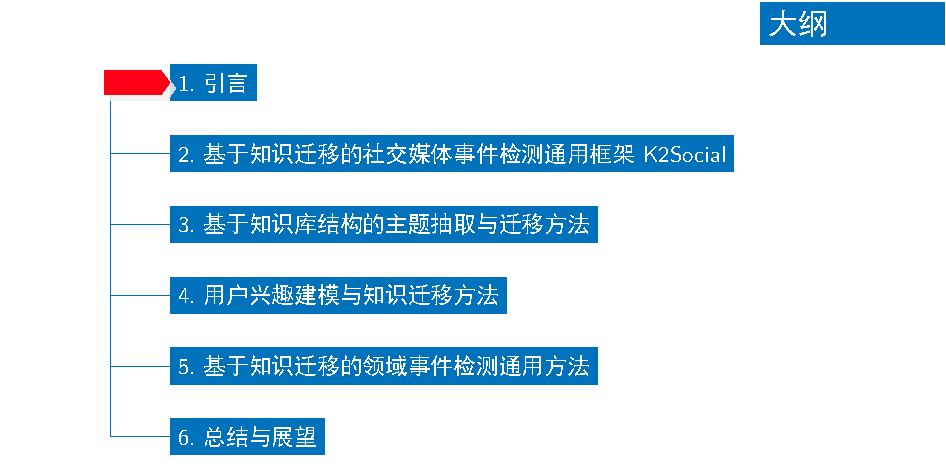
\includegraphics[width=1.0\paperwidth]{img/contents1_output.pdf}
\end{figure}
\end{frame}
\end{withoutheadline}

\section{引言}
%------------------------------
%\begin{frame}
%\frametitle{社交媒体事件检测问题的背景}
%
%\begin{figure}
%    
\includegraphics[width=0.75\paperwidth]{img/logos.pdf}
%\end{figure}
%
%\end{frame}


%------------------------------
\begin{frame}
\frametitle{\noindent 社交媒体事件检测问题的背景}
社交媒体上进行事件检测可服务于众多应用:
\begin{figure}
    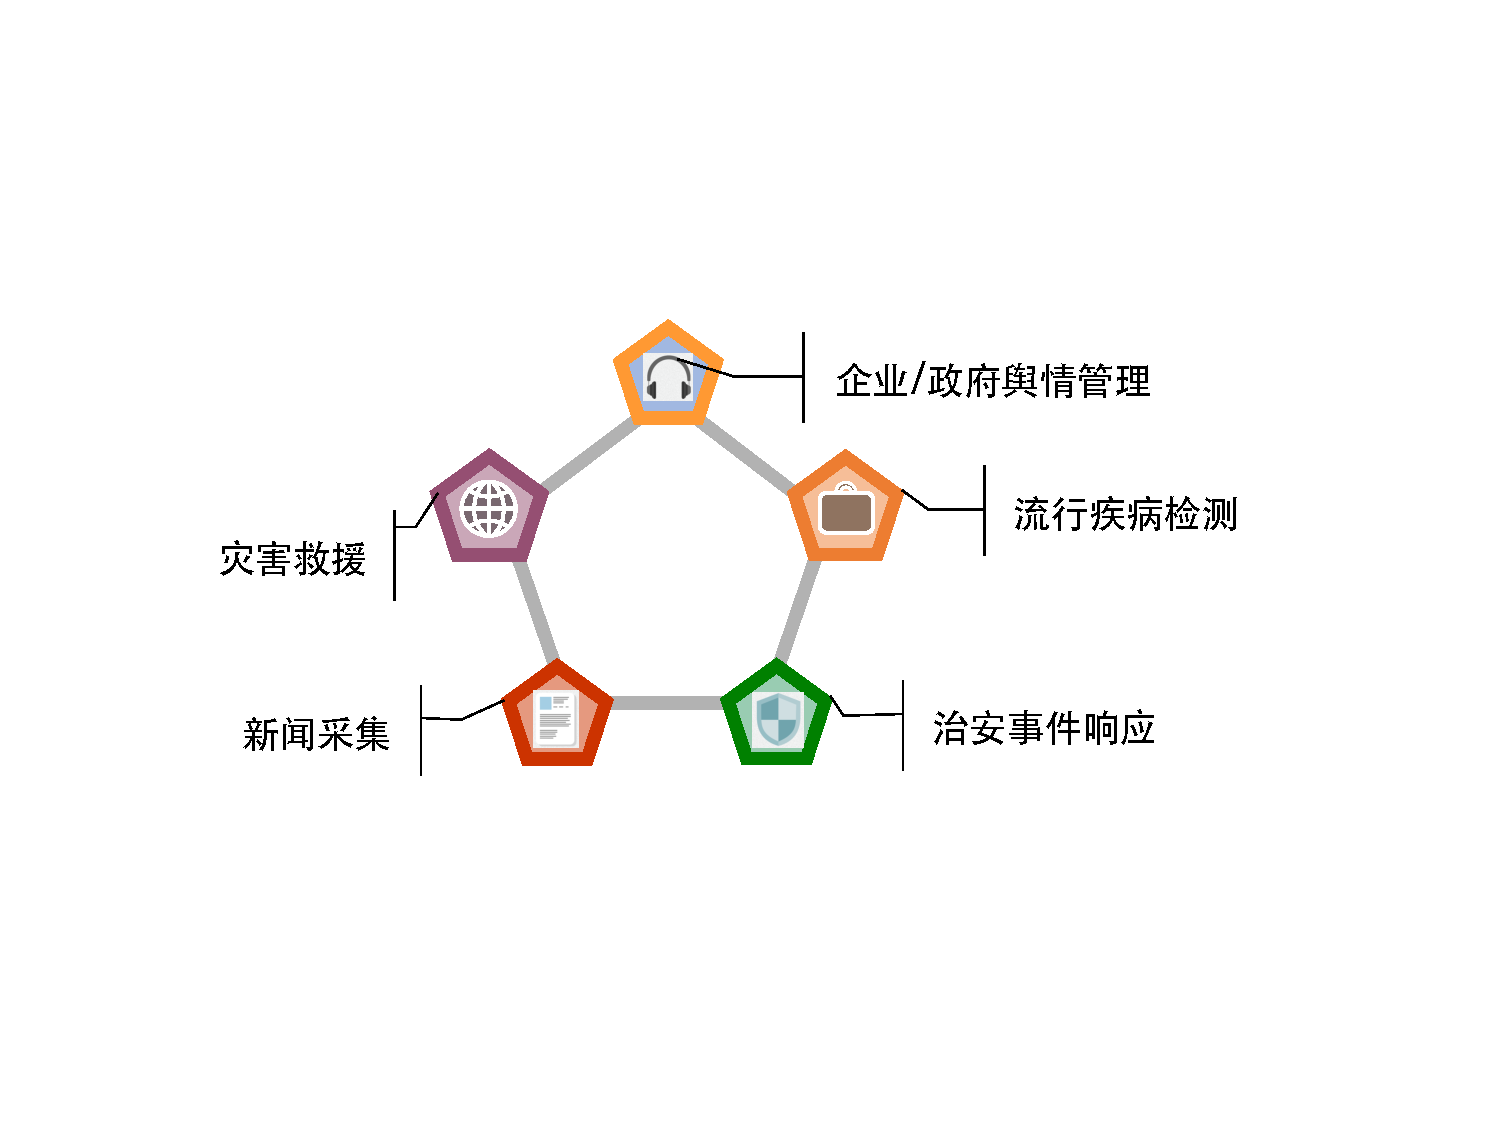
\includegraphics[width=0.75\paperwidth]{img/event_applications.pdf}
\end{figure}

\end{frame}

\begin{frame}
\frametitle{\noindent 社交媒体事件检测问题的背景}	
科研项目背景:
\begin{enumerate}
	\item 非结构化数据管理系统北大部分——国家“核高基”重大专项(2010ZX01042-002-002-02)
	\item 海量Web数据结构化内容提取与集成及大型示范应用——国家863计划课题(2012AA011002)
	\item 微博用户社区及主题时序方法研究——中国信息安全测评中心合作项目
\end{enumerate}
\end{frame}


%------------------------------
\begin{frame}
\frametitle{\noindent 社交媒体的语境动态演变及带来的挑战}
%\onslide<1-4>{
\begin{tcolorbox}[colback=red!5,colframe=red!75!black]
社交媒体用语不规范,主题动态变化,我们将其总结为社交媒体的语境动态演变
\end{tcolorbox}
%}

\vspace{-5mm}

\begin{columns}[onlytextwidth, t]
\column{0.32\linewidth}
%	\onslide<2-4>{
    \begin{tcolorbox}[colback=red!5,colframe=red!5]
    交流语境的变化:从正式交流语境到非正式交流语境的转变,导致用语不规范[Gunraj 2016].
    \end{tcolorbox}
%    }

\column{0.32\linewidth}
%	\onslide<3-4>{
    \begin{tcolorbox}[colback=red!5,colframe=red!5]
    外部语境的变化:用户易于被外界影响[Weng 2012],热门话题随着时间快速变化。
    \end{tcolorbox}
%    }
    
\column{0.32\linewidth}
%	\onslide<4>{
    \begin{tcolorbox}[colback=red!5,colframe=red!5]
    前述两种变化的综合叠加,例子:Somehow made it through Irene. 仅在2011.8的语境中知道这是关于飓风艾琳。 
    \end{tcolorbox}
%    }
\end{columns}

%\begin{tcolorbox}[colback=red!5,colframe=red!75!black]
%外在表现:用语不规范,主题动态变化
%\end{tcolorbox}
\end{frame}

\begin{frame}
\frametitle{\noindent 相关研究状况}

    \begin{tcolorbox}[colback=red!5,colframe=red!5]
传统媒体中事件的定义[Allan, 2002]:在特定的时间,特定的地点发生的特定的事,以及其附属的前提条件和后续结果,称作事件。\\
社交媒体中事件的定义[Becker, 2011]:仅当上述定义中的事件被社交媒体报道了才能被定义为社交媒体上的事件。    \end{tcolorbox}

\centering{\color{blue}$\Downarrow$} 形式化定义

    \begin{tcolorbox}[colback=red!5,colframe=red!5]
    社交媒体上的事件\(e\)由社交媒体数据流\(D_e=(d_{e,1}, d_{e,2}, \) \(\cdots, d_{e,m})\)确定:在时间窗口\([t_{e,1}, t_{e,m}]\) 上,\(D_e\)的文本集合\(w_{e,1}, \cdots ,w_{e,m}\)确定出的{\color{red}特征项}的频率明显高于时刻\(t_{e,1}\)之前该特征项频率的期望值,且\(D_e\)能够对应于现实中在特定时间已发生的特定的事。
	\end{tcolorbox}


\end{frame}


%------------------------------
\begin{frame}
\frametitle{\noindent 相关研究状况}
\vspace{-1cm}
\begin{table}[]
\centering
\caption{社交媒体事件检测已有方法}
\scalebox{0.75}{
\begin{tabular}{|c|c|c|c|c}
\cline{1-4}
方法类型 & 代表工作 & 事件粒度 & 特点 &  \\ \cline{1-4}
基于普通聚类的方法 & {[}Chen, SIGIR 2013{]} & 高频的相似微博 & 实现简单 &  \\ \cline{1-4}
基于敏感哈希的方法 & {[}Petrovic, NAACL 2010{]} & 高频的相似微博 & 响应速度快 &  \\ \cline{1-4}
基于词频统计的方法 & {[}HE,SIGIR 2007{]} & 高频词组 & \begin{tabular}[c]{@{}l@{}}可区分周期性、\\ 非周期性事件\end{tabular} &  \\ \cline{1-4}
基于主题模型的方法 & \begin{tabular}[c]{@{}l@{}}{[}Yan, AAAI 2015{]}\\ {[}Jahnichen, AISTATS 2018{]}\end{tabular} & 主题 & 可利用上下文信息 &  \\ \cline{1-4}
基于分类器+后处理 & {[}Yang, KDD 2014{]} & \begin{tabular}[c]{@{}l@{}}对微博分类后,\\ 再检测事件\end{tabular} & 进行领域事件检测 &  \\ \cline{1-4}
\end{tabular}
}
\end{table}

{\color{blue} 受限于社交媒体的语境动态演变,上述方法难于准确检测事件。}
\end{frame}
%%TODO 制作导航部分
\begin{withoutheadline}
\begin{frame}
\vspace*{-13mm}
\begin{figure}
	\hspace*{-4.2mm}
    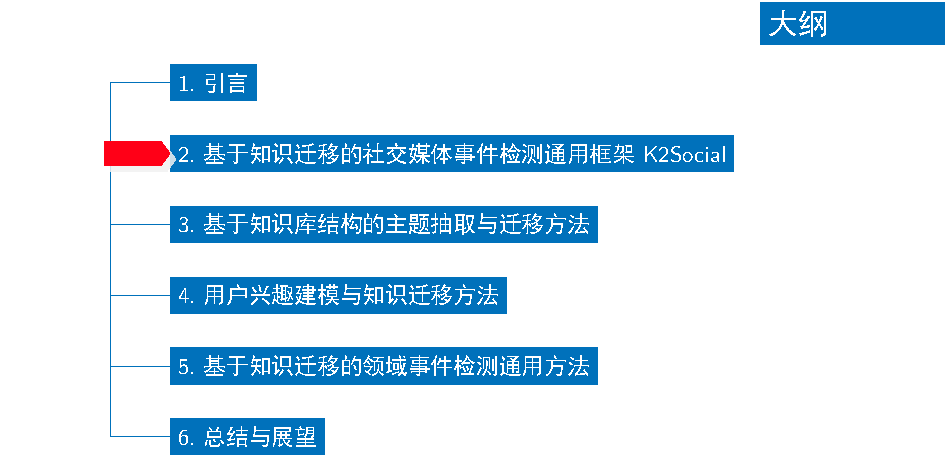
\includegraphics[width=1.0\paperwidth]{img/contents2_output.pdf}
\end{figure}

\end{frame}
\end{withoutheadline}

\section{基于知识迁移的社交媒体事件检测通用框架K2Social}
%------------------------------
%page 2
\begin{frame}
%\frametitle{Motivation}
\vspace*{-2mm}
\begin{figure}
    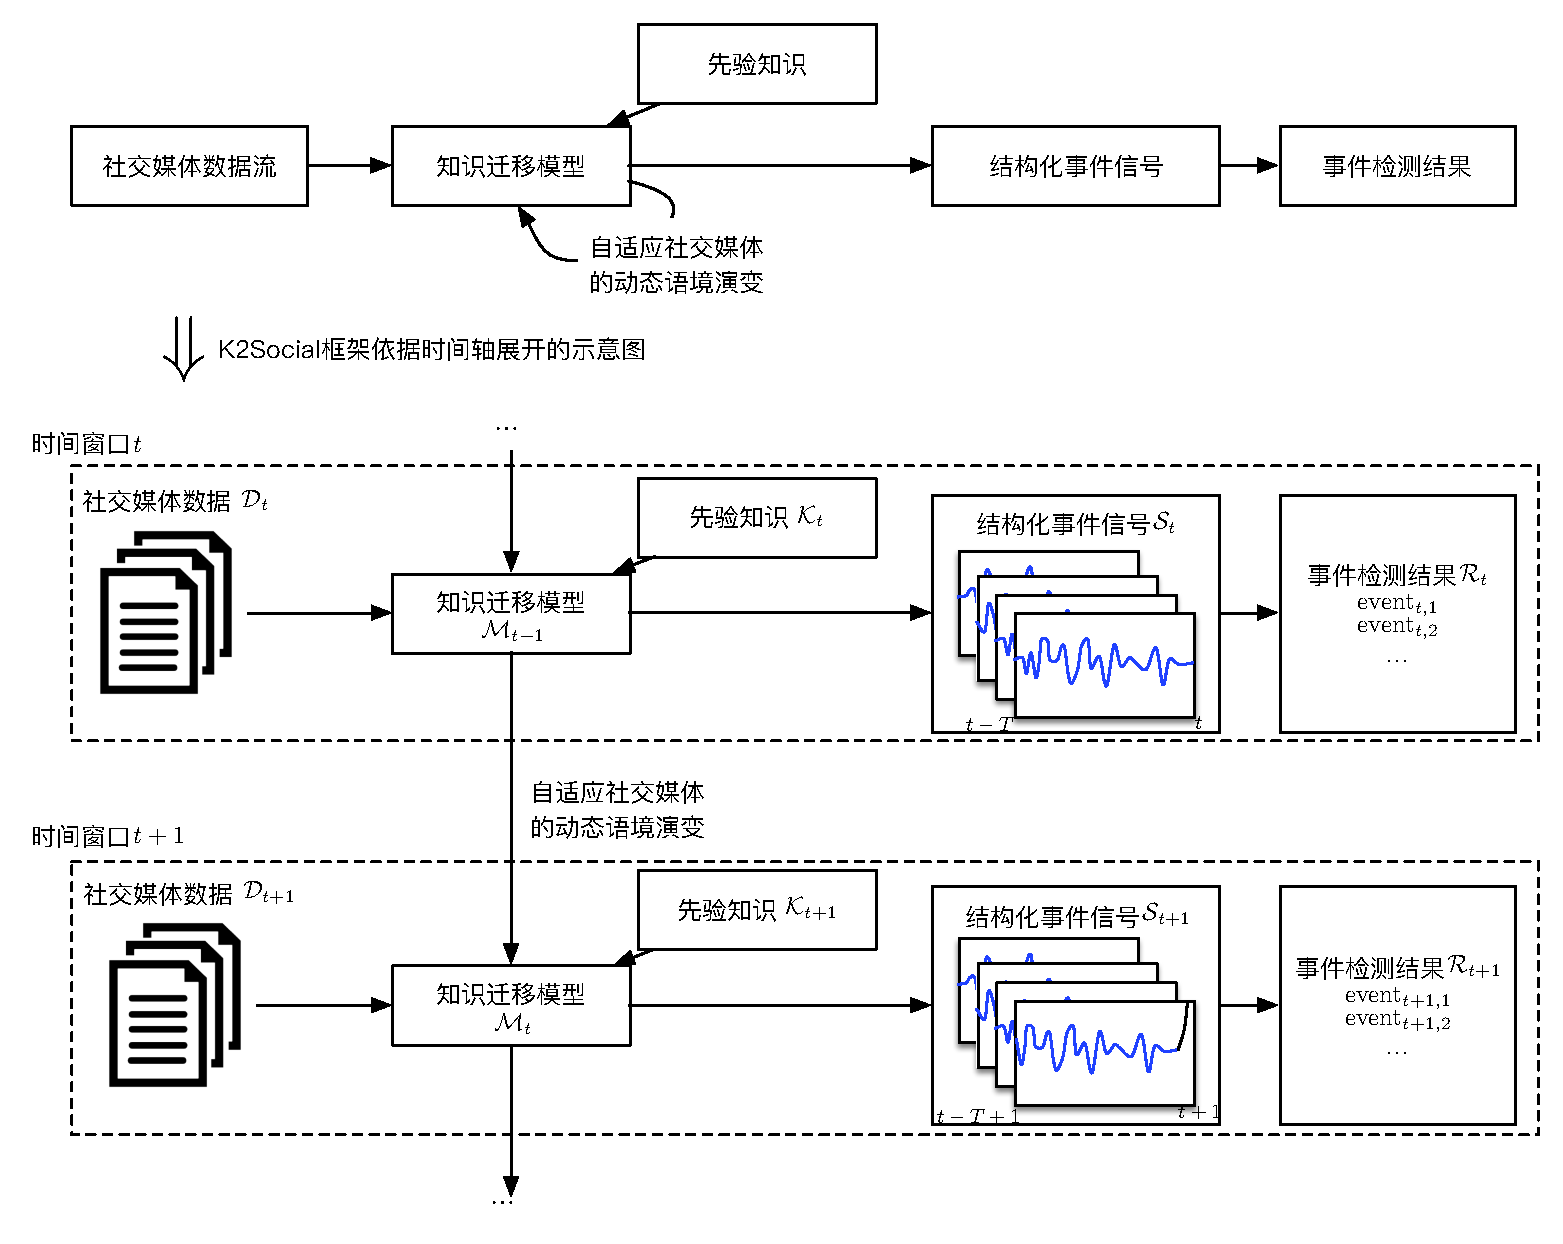
\includegraphics[width=0.66\paperwidth]{img/K2Social_flow}
\end{figure}

\end{frame}


\include{chaps/chapTmp_frame}
%%TODO 制作导航部分
\begin{withoutheadline}
\begin{frame}
\vspace*{-13mm}
\begin{figure}
	\hspace*{-4.2mm}
    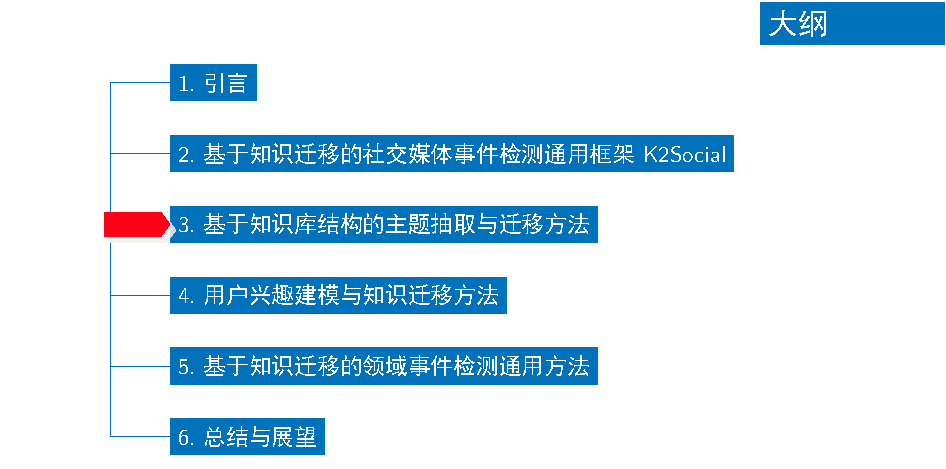
\includegraphics[width=1.0\paperwidth]{img/contents3_output.pdf}
\end{figure}

\end{frame}
\end{withoutheadline}

\section{基于知识库结构的主题抽取与迁移方法}
\begin{frame}
%\frametitle{\textsc{TransDetector}: Phase 1 (Extracting Category-Level Topics in KB) (3/3)}	
%Taking the category \textit{Military} as an example, we extract \textit{Military}'s category-level topic \(\bm{h_{Military}}\).
\begin{figure}[h]
		\setlength{\abovecaptionskip}{0.cm}
        \setlength{\belowcaptionskip}{0.cm}
        \centering
        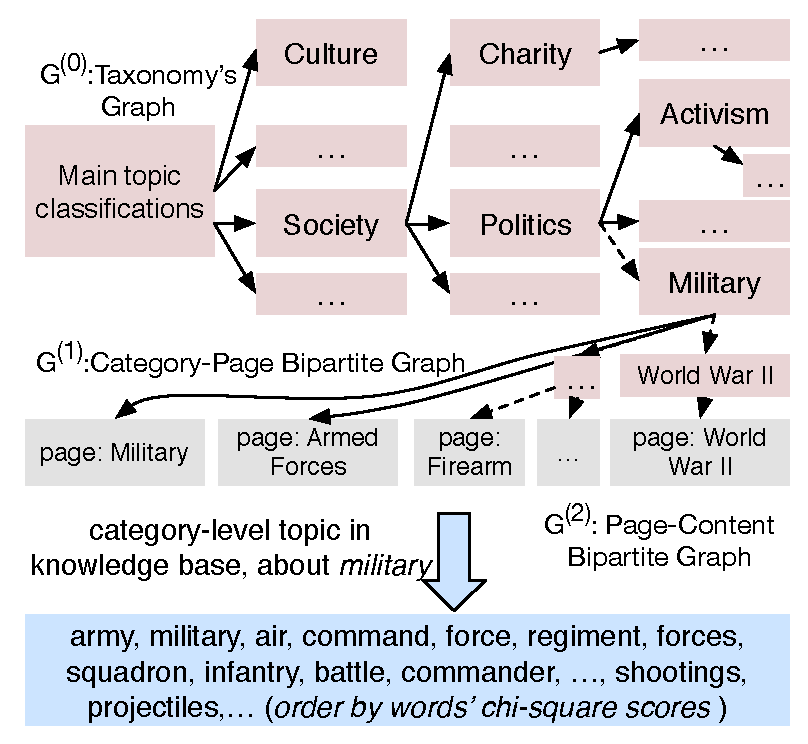
\includegraphics[width=0.7\columnwidth]{img/initializationExample.pdf}
        %\caption{Extracting Category-Level Topics in Knowledge Base via its three fold hierarchical structure, taking \textit{Military} as an example.}
        \label{fig:hood}
\end{figure}
\end{frame}

\begin{frame}
\frametitle{\textsc{TransDetector}: Phase 2 (Transferring Category-Level Info into Microblog Stream) (1/2)}	
Transfer KB's Category-Level Topics \(\{\bm{h_c}\}_{c=1}^{K_{KB}}\) into microblogs stream: CTrans-LDA.
\begin{figure}[h]
		\setlength{\abovecaptionskip}{0.cm}
        \setlength{\belowcaptionskip}{0.cm}
        \centering
        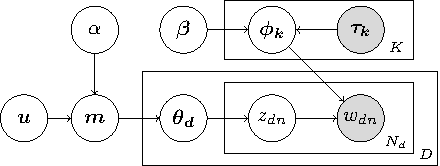
\includegraphics[width=0.6\columnwidth]{img/lda_tikz.pdf}
        \caption{Diagram of CTrans-LDA.}
        \label{fig:hood}
\end{figure}

In CTrans-LDA, \(\{\bm{h_c}\}_{c=1}^{K_{KB}}\) is used as prior information:
\setlength{\abovedisplayskip}{0pt}
\setlength{\belowdisplayskip}{0pt}
\begin{scriptsize}
\begin{equation}
\label{eq:wikiPrior}
\begin{aligned}
\tau_{kv}=
\left\{ \begin{aligned}
\lambda \frac{h_{kv}}{\sum_{v\in S_{k}}h_{kv}} &,v\in S_{k}\ and  \ k \leq K_{\bm{KB}} \\
0&,v \notin S_{k} \ or \ k > K_{\bm{KB}} \\
\end{aligned}\right.
\end{aligned}
\end{equation}
\end{scriptsize}
\end{frame}

\begin{frame}
\frametitle{\textsc{TransDetector}: Phase 2 (Transferring Category-Level Info into Microblog Stream) (2/2)}	
We use Gibbs Sampling for solving CTrans-LDA.
\begin{itemize}
	\item The initialization probability \(\hat{q}_{k|v}\) makes sure that the learned topics are aligned to the pre-defined category-level topic.
\setlength{\abovedisplayskip}{0pt}
\setlength{\belowdisplayskip}{0pt}
\begin{scriptsize} 
\begin{equation}
\label{eq:initProbability}
\begin{aligned}
\hat{q}_{k|v}=
\left\{ \begin{aligned}
\frac{\tau_{kv}}{\sum_{k=1}^{K}\tau_{kv}} &,\sum_{k}\tau_{kv}>0 & (a)\\
0&, \sum_{k}\tau_{kv}=0 \ and \ k \leq K_{\bm{KB}} & (b)\\
1/(K-K_{\bm{KB}})&,\sum_{k}\tau_{kv}=0 \ and \ k > K_{\bm{KB}} & (c)
\end{aligned}\right.
\end{aligned}
\end{equation}
\end{scriptsize}
\item Conditional probability in gibbs sampling:
\(p(z_{dn}=k|.)\propto (n^{(d)}_{dk}+\alpha m_k)(n^{(w)}_{kv}+\tau_{kv}+\beta)/(n^{(w)}_{k,.}+\tau_{k,.}+V\beta)\).
\end{itemize}
\end{frame}


\begin{frame}
\frametitle{\textsc{TransDetector}: Phase 3 (Detecting Events on Category-Level Word Time Series) (1/2)}	
After transfer learning, we conduct analysis on category-level word time series, and detect events in microblog stream.
\begin{figure}[h]
		\setlength{\abovecaptionskip}{0.cm}
        \setlength{\belowcaptionskip}{0.cm}
        \centering
        \caption{Visualizing Category-Level Word Time Series in Microblog Stream on Edinburgh Twitter Corpus (20110711-20110915), taking \textit{Military} as an example.}
        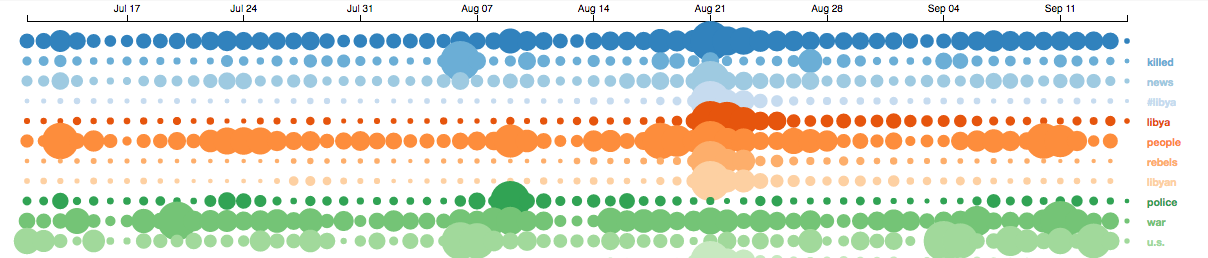
\includegraphics[width=.99\columnwidth]{img/screenShot.png}
        \label{fig:hood}
\end{figure}
\end{frame}


\begin{frame}
\frametitle{实验结果:基于知识库结构的主题抽取质量}	

\begin{table}[h]
\setlength{\abovecaptionskip}{0.cm}%set the distance between caption and table to 0 cm.
\setlength{\belowcaptionskip}{0.cm}
\centering
\caption{以\textit{Aviation}概念类别为例,\textsc{TransDetector}抽取的相关主题与LightLDA(取主题个数为100)抽取的相关主题在主题连贯性(NPMI)指标上的对比。}
\scalebox{0.45}{
\begin{tabular}{|c|l|l|c !{\vrule width 1pt} c|l|l|c|}
\hline
\multicolumn{4}{|c!{\vrule width 1pt}}{Category-Level Topics extracted from Wikipedia by \textsc{TransDetector}} & \multicolumn{4}{c|}{Topics Learned from Wikipedia by LightLDA}    \\ \hline
GID& \#words*  & words  & NPMI & GID& \#words*& words & NPMI \\ \hline
- & 1-5 & aircraft air airport flight airline &-& - & 1-5 & engine aircraft car air power &-\\ \hline
0 & 1-5, 6-10 & \(\sim\), airlines aviation flying pilot squadron &  0.113 & 0 & 1-5, 6-10 & \(\sim\), design flight model production speed & 0.112\\ \hline
1 & 1-5, 11-15 & \(\sim\), flights pilots raf airways fighter & 0.155 & 1 & 1-5, 11-15 &\(\sim\), system vehicle cars engines mm & 0.062\\ \hline
2 & 1-5, 16-20 & \(\sim\), boeing runway force crashed flew   & 0.092 & 2 & 1-5, 16-20 & \(\sim\), fuel vehicles designed models type & 0.072\\ \hline
3 & 1-5, 21-25 &\(\sim\), airfield landing passengers plane aerial & 0.179 & 3 & 1-5, 21-25 & \(\sim\), version front produced rear electric & 0.035\\ \hline
4 & 1-5, 26-30 &\(\sim\), bomber radar wing bombers crash & 0.137 & 4 & 1-5, 26-30 & \(\sim\), space control motor standard development & 0.085\\ \hline
5 & 1-5, 31-35 &\(\sim\), airbus airports operations jet helicopter & 0.189 & 5 & 1-5, 31-35 & \(\sim\), film range light using available & -0.002\\ \hline
6 & 1-5, 36-40 &\(\sim\), squadrons base flown havilland crew & 0.088 & 6 & 1-5, 36-40 & \(\sim\), wing powered wheel weight launch & 0.087\\ \hline
7 & 1-5, 41-45 & \(\sim\), combat luftwaffe aerodrome carrier fokker & 0.159 & 7 & 1-5, 41-45 & \(\sim\), developed low test ford cylinder & 0.007\\ \hline
8 & 1-5, 46-50 &\(\sim\), planes fly engine takeoff fleet & 0.186 & 8 & 1-5, 46-50 & \(\sim\), equipment side pilot hp aviation & 0.091\\ \hline
9 & 1-5, 51-55 &\(\sim\), fuselage helicopters aviator naval aero & 0.157 & 9 & 1-5, 51-55 & \(\sim\), systems us sold body drive & -0.051\\ \hline
10 & 1-5, 56-60 &\(\sim\), glider command training balloon faa & 0.166 & 10 & 1-5, 56-60 & \(\sim\), gear introduced class safety seat & 0.069\\ \hline
\(\cdots\) & \(\cdots\) &\(\cdots\) &\(\cdots\) & \(\cdots\) & \(\cdots\) &\(\cdots\) &\(\cdots\)\\ \hline
18 & 1-5, 96-100 &\(\sim\), scheduled carriers military curtiss biplane &0.131 & 18 & 1-5, 96-100 & \(\sim\), transmission special replaced limited different & 0.059\\ \hline
19 & 1-5, 101-105 &\(\sim\), accident engines iaf albatross rcaf &0.068 & 19 & 1-5, 101-105 & \(\sim\), features machine nuclear even unit & 0.011\\ \hline
\end{tabular}
}
\label{tbl:NPMIDetails}
\end{table}

\end{frame}


\begin{frame}
\frametitle{实验结果:基于知识库结构的主题抽取质量}	
\begin{figure}[h]
	\setlength{\abovecaptionskip}{0.cm}
	\setlength{\belowcaptionskip}{0.cm}
        \centering
		\caption{对更多的\textsc{TransDetector}从维基百科抽取的概念类相关的主题的连贯性与LightLDA在维基百科上学习的主题连贯性进行对比。在前10个分组上,\textsc{TransDetector}显著更优。}
        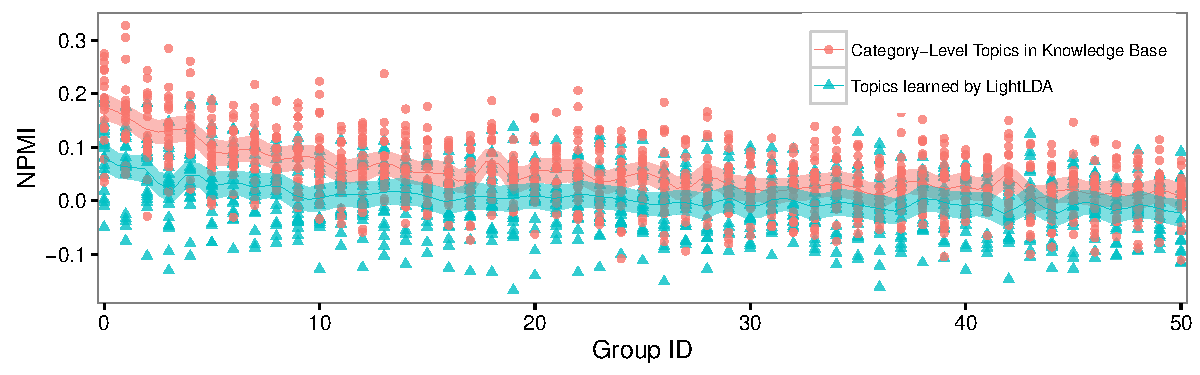
\includegraphics[width=1.0\columnwidth]{img/NPMI.pdf}
        \label{fig:NPMI}
\end{figure}
\end{frame}



%------------------------------
%page 2
\begin{frame}
\frametitle{实验结果:迁移学习效果}
\begin{table}
\setlength{\abovecaptionskip}{0.cm}%set the distance between caption and table to 0 cm.
\setlength{\belowcaptionskip}{0.cm}
\centering
\caption{CTrans-LDA迁移学习效果示例,展示从知识库中抽取的主题和经过迁移学习后微博中相关的主题。斜体标注的词为经过迁移学习后在\textit{社交媒体域}中学习到的和概念类别相关的新词。}
\scalebox{0.55}{
\begin{tabular}{|cc|cc|cc|cc|cc|cc|}
\hline
\multicolumn{2}{|c|}{\textit{Aviation}} & \multicolumn{2}{c|}{\textit{Health}} & \multicolumn{2}{c|}{\textit{Middle East}} & \multicolumn{2}{c|}{\textit{Military}} & \multicolumn{2}{c|}{\textit{Mobile Phones}}\\
\begin{tabular}[c]{@{}c@{}}Knowledge\\ Base\end{tabular} & \begin{tabular}[c]{@{}c@{}}Microblog\\ Stream\end{tabular} & \begin{tabular}[c]{@{}c@{}}Knowledge\\ Base\end{tabular} & \begin{tabular}[c]{@{}c@{}}Microblog\\ Stream\end{tabular} & \begin{tabular}[c]{@{}c@{}}Knowledge\\ Base\end{tabular} & \begin{tabular}[c]{@{}c@{}}Microblog\\ Stream\end{tabular} & \begin{tabular}[c]{@{}c@{}}Knowledge\\ Base\end{tabular} & \begin{tabular}[c]{@{}c@{}}Microblog\\ Stream\end{tabular} & \begin{tabular}[c]{@{}c@{}}Knowledge\\ Base\end{tabular} & \begin{tabular}[c]{@{}c@{}}Microblog\\ Stream\end{tabular} \\ 
\hline
aircraft & air & health & weight & al & \textbf{\textit{\#syria}} & army & killed & android & iphone\\ 
air & plane & patients & loss & israel & \textbf{\textit{\#bahrain}} & military & news & mobile & apple \\ 
airport & flight & medical & diet & iran & people & air & \textbf{\textit{\#libya}} & nokia & android \\ 
flight & time & disease & health & arab & israel & command & libya & ios & app \\
airline & airlines & treatment & cancer & israeli & police & force & rebels & phone & ipad \\
airlines & news & hospital & lose & egypt & \textbf{\textit{\#libya}} & regiment & people & samsung & samsung \\
aviation & boat & patient & fat & egyptian & \#egypt & forces & police & game & mobile\\
flying & airport & clinical & tips & ibn & news & squadron & war & app & blackberry \\
pilot & force & symptoms & treatment & jerusalem & \textbf{\textit{\#israel}} & infantry & libyan & iphone & tablet \\
squadron & fly & cancer & body & syria & world & battle & attack & htc & apps\\
\hline
\end{tabular}
}
\label{tbl:historyStates}
\end{table}
\end{frame}


\begin{frame}
\frametitle{实验结果:事件检测效果}	
\noindent \textsc{TransDetector}在保证召回率的同时,将准确率提升9\%

\begin{table}[h]
\setlength{\abovecaptionskip}{0.cm}%set the distance between caption and table to 0 cm.
\setlength{\belowcaptionskip}{0.cm}
\centering
\caption{在基于\textit{Edinburgh twitter corpus}数据集上构建的Benchmark1和Benchmark2,各个事件检测方法的性能对比}
\scriptsize
\scalebox{0.75}{
\begin{threeparttable}  
\begin{tabular}{|c|c|c|c|c|c|c|}
    \hline
    Method & \begin{tabular}[c]{@{}c@{}}Number of\\Events to \\ be Evaluated \end{tabular} & \begin{tabular}[c]{@{}c@{}}Recall@ \\ Benchmark1\end{tabular}& \begin{tabular}[c]{@{}c@{}}Precision@ \\ Benchmark2\end{tabular} & \begin{tabular}[c]{@{}c@{}}Recall@ \\ Benchmark2\end{tabular} & \begin{tabular}[c]{@{}c@{}}F@ \\ Benchmark2\end{tabular} & \begin{tabular}[c]{@{}c@{}}DERate\tnote{a}\ \ (Duplicate\\ Event Rate)@\\ Benchmark2\end{tabular} \\ \hline
    LSH & 500 & 0.704 & 0.788 & 0.651 & 0.713 & 0.348 \\ \hline
    TimeUserLDA & 100 & 0.370 & 0.790 & 0.177 & 0.289 & 0.114 \\ \hline
    Twevent & 375 &  0.741 & 0.808 & 0.658 & 0.725 & 0.142 \\ \hline
    EDCoW & 349 & 0.556 & 0.748 & 0.511 & 0.607 & 0.226 \\ \hline
    BurstyBTM & 200 & 0.667 & 0.825 & 0.384 & 0.497 & \textbf{0.079} \\ \hline
    \textsc{TransDetector} & 457 & \textbf{0.889} & \textbf{0.912} & \textbf{0.876} & \textbf{0.894} & 0.170 \\ \hline
    \end{tabular}

\begin{tablenotes}  
\item[a] DERate = (the number of duplicate events) / (the total number of detected realistic events)
\end{tablenotes}  
\end{threeparttable}  
}
\label{tbl:overall}
\end{table}
\end{frame}


\begin{frame}
\frametitle{实验结果:事件检测效果}
\noindent \textsc{TransDetector}在较小规模的事件上召回率明显高于已有方法。
\vfill
\begin{figure}[h]
	\setlength{\abovecaptionskip}{0.cm}
	\setlength{\belowcaptionskip}{0.cm}
        \centering
        \caption{在基于\textit{Edinburgh twitter corpus}数据集构建的Benchmark2上,召回率与事件规模之间的关系示意图}
        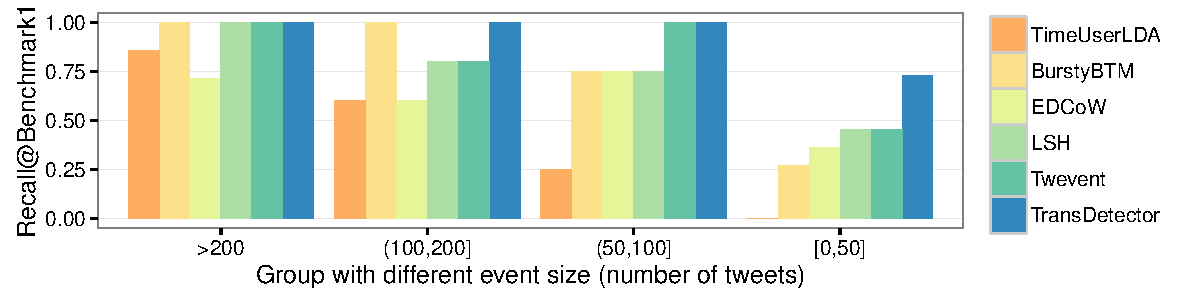
\includegraphics[width=1.0\columnwidth]{img/barchartOnBenchmark1.pdf}
        \label{fig:Benchmark1}
\end{figure}
\end{frame}

\begin{frame}
\frametitle{实验结果:事件检测效果}	
\noindent \textsc{TransDetector}在较小规模的事件上召回率明显高于已有方法。
\begin{table}
\setlength{\abovecaptionskip}{0.cm}%set the distance between caption and table to 0 cm.
\setlength{\belowcaptionskip}{0.cm}
\centering
\caption{2011-07-22至2011-07-28,\textit{Edinburgh Twitter Corpus}数据集中军事相关事件列表以及各事件检测方法的具体表现}
\vspace{-0.5cm}
\scalebox{0.6}{
\begin{threeparttable}  
\begin{tabular}{|c|l|l|c|c|c|c|c|c|c|}
\hline
\multirow{2}{*}{Date} & \multirow{2}{*}{Event key words} & \multirow{2}{*}{Representative event tweet} & \multirow{2}{*}{\begin{tabular}[c]{@{}l@{}}Number of \\ event tweet\end{tabular}} & \multicolumn{6}{c|}{Methods\tnote{a}} \\ \cline{5-10} 
 &  &  &  & L & TU & TW & E & B & TD \\ \hline
7/22/11 & \begin{tabular}[c]{@{}l@{}}Norway, Oslo,\\ attacks, bombing\end{tabular} & \begin{tabular}[c]{@{}l@{}}Terror Attacks Devastate Norway: A bomb\\ ripped through government offices in Oslo \\and a gunman... http://dlvr.it/cLbk8\end{tabular} & 557 & \checkmark & \checkmark & \checkmark & \checkmark & \checkmark & \checkmark \\ \hline
7/23/11 & Gunman, rink & \begin{tabular}[c]{@{}l@{}}Gunman Kills Self, 5 Others at Texas Roller\\ Rink http://dlvr.it/cLcTH\end{tabular} & 43 & - & - & \checkmark &  \checkmark & - & \checkmark \\ \hline
7/26/11 & \begin{tabular}[c]{@{}l@{}}Kandahar, mayor, \\ suicide, attack\end{tabular} & \begin{tabular}[c]{@{}l@{}}TELEGRAPH{]}: Kandahar mayor killed by\\ Afghan suicide bomber: The mayor of \\Kandahar, the biggest city in south \_\end{tabular} & 47 & \checkmark & - & \checkmark & \checkmark & - & \checkmark \\ \hline
7/28/11 & Ft., Hood, attack & \begin{tabular}[c]{@{}l@{}} Possible Ft. Hood Attack Thwarted\\ http://t.co/BSJ33hk\end{tabular} & 52 & - & - & - & - & - & \checkmark \\ \hline
7/28/11 & \begin{tabular}[c]{@{}l@{}}Libyan, rebel, \\ gunned\end{tabular} & \begin{tabular}[c]{@{}l@{}}Libyan rebel chief gunned down in Benghazi \\ http://sns.mx/prfvy1\end{tabular} & 44 & - & - & - & - & - & \checkmark \\ \hline
\end{tabular}

\begin{tablenotes}  
\item[a] L=LSH, TU=TimeUserLDA, TW=Twevent, E=EDCoW, B=BurstyBTM, TD=\textsc{TransDetector}.
\end{tablenotes}  
\end{threeparttable}  
}
\end{table}
\end{frame}

\begin{frame}
\frametitle{TransDetector方法小结}
\begin{columns}
\column{0.75\textwidth}

\begin{enumerate}
	\item 提出了一种以知识库结构为导向的概念类相关的主题抽取方法;
	\item 提出了新的概率主题模型CTrans-LDA用于知识的迁移,并能自适应社交媒体的语境动态演变;
	\item 在知识迁移后的时间序列上进行事件检测,准确地检测社交媒体中蕴含的事件;
	\item Edinburgh Twitter Corpus数据集上准确率相较于目前已有的最佳方法提升了9\%
\end{enumerate}

\column{0.75\textwidth}

\end{columns}

\end{frame}

\begin{withoutheadline}
\begin{frame}
\vspace*{-13mm}
\begin{figure}
	\hspace*{-4.2mm}
    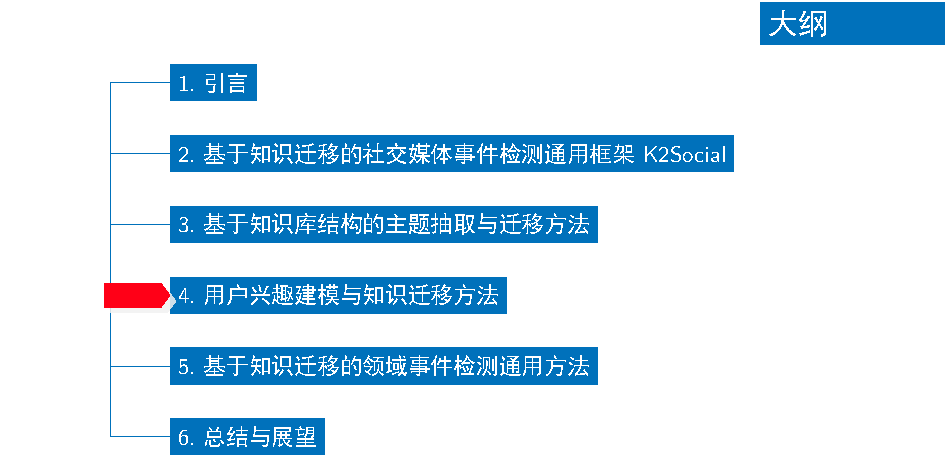
\includegraphics[width=1.0\paperwidth]{img/contents4_output.pdf}
\end{figure}

\end{frame}
\end{withoutheadline}

\section{用户兴趣建模与知识迁移方法}

%------------------------------
%TODO 要说明对突发事件检测有迫切需求
\begin{frame}
\frametitle{Motivation}	
issue
说明对突发事件检测有迫切需求

\pdfnote{前面一节中已经分析了知识迁移对事件检测准确性的提升,这一小节中我们分析知识迁移对事件检测时效性的提升}
\end{frame}

\begin{frame}
\frametitle{突发事件的特点}
这里放一幅插图,说明突发事件的特点是不同兴趣的用户在同一时间窗口内都关心的事件。
\pdfnote{突发事件的特点是不同兴趣的用户在同一时间窗口内都关心的事件。}
\end{frame}

%------------------------------
\begin{frame}
\frametitle{Motivation}
\begin{figure}[h]
		\setlength{\abovecaptionskip}{0.cm}
        \setlength{\belowcaptionskip}{0.cm}
        \centering
		\caption{社交媒体关注网络用于扩充个人自我描述信息示意图}
        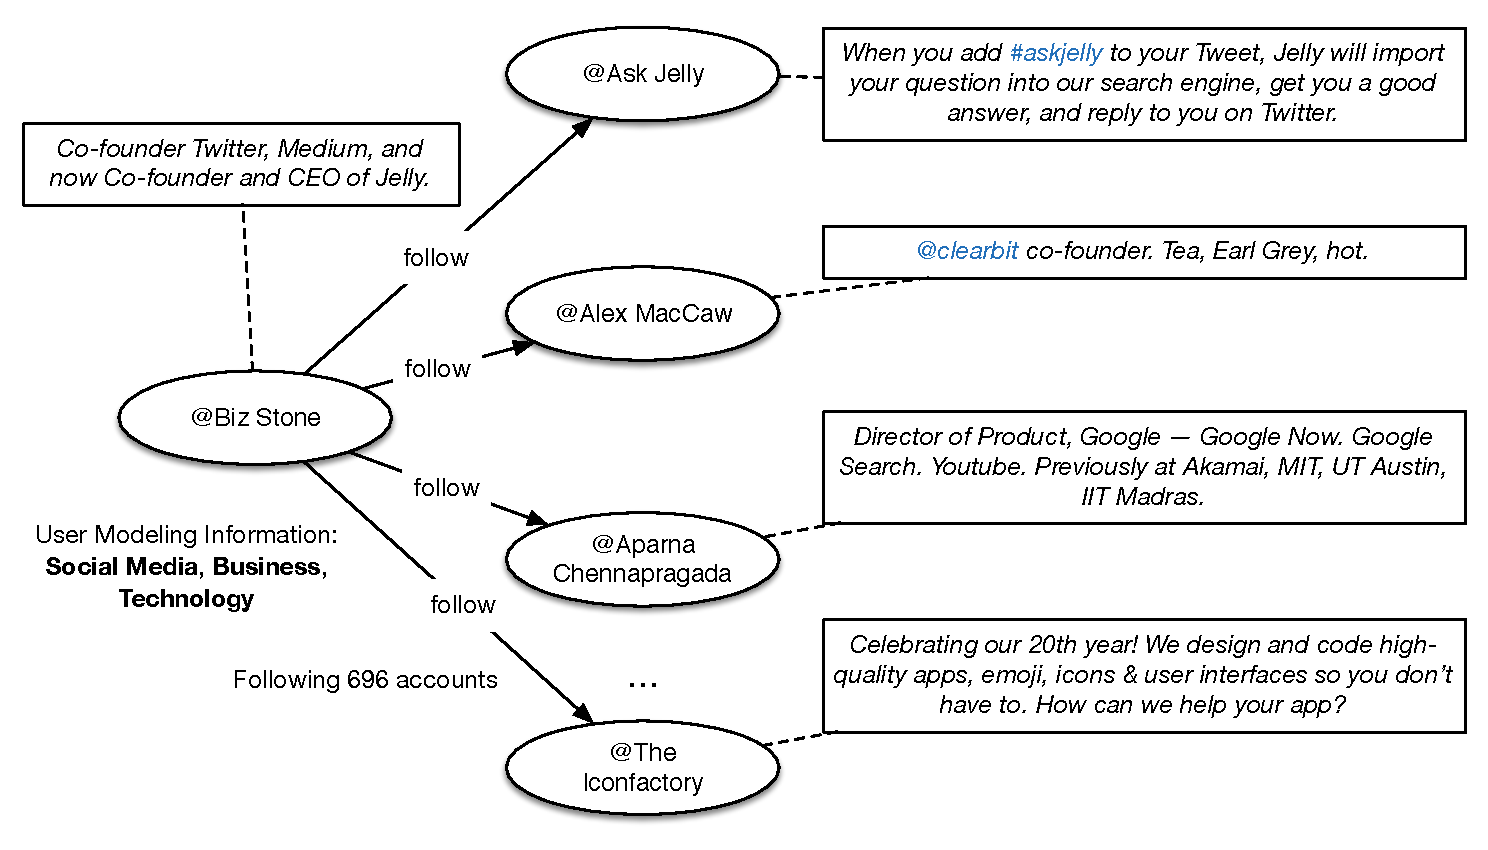
\includegraphics[width=0.9\columnwidth]{img/UMIETM/UMIETM_profile.pdf}
\end{figure}
\end{frame}

%------------------------------
\begin{frame}
\frametitle{我们的方法}
UMIETM模型(User Modeling Based Interest and Event Topic Modeling)
\begin{itemize}
\item 使用用户个人描述信息与用户关注网络建模用户兴趣分布
\item 将用户兴趣知识迁移到微博中
\item 区分用户兴趣与突发事件
\end{itemize}

\vspace{-3mm}
\begin{figure}
	\setlength{\abovecaptionskip}{0.cm}
	\setlength{\belowcaptionskip}{0.cm}
	\caption{UMIETM概率模型}
	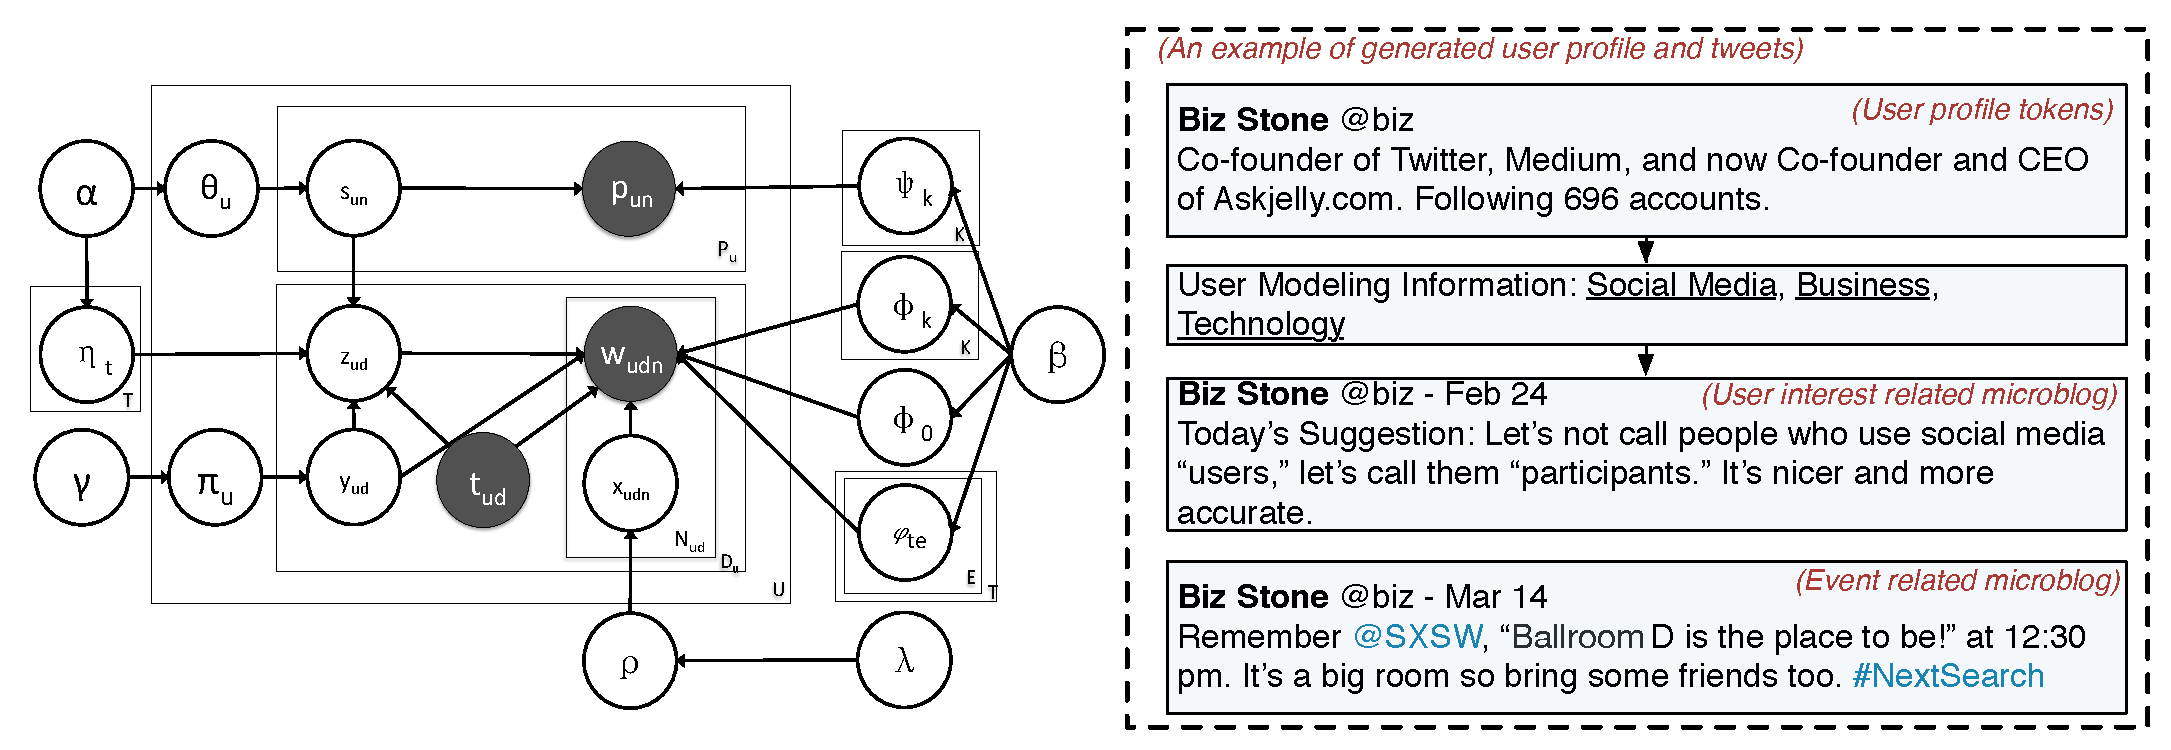
\includegraphics[width=1.0\textwidth]{img/UMIETM/model.pdf}
	\label{fig:modelUMIETM}
\end{figure}
\pdfnote{(左侧)UMIETM概率模型示意图。(右侧)示例用户Biz Stone的两类文本(用户兴趣相关的文本与突发事件相关的文本)的示意图。其个人简档揭示出其个人兴趣主要集中在社交网络、商业、科技领域。依据UMIETM模型,可以检测出他2016年2月24日发布的有关社交网络中用户角色定位的文本可以被检测为与个人兴趣相关;2016年3月14日发布的有关SXSW的文本则与个人兴趣都不相关,结合该时间窗口内更多的其他文本,可以将判断这条文本和突发事件相关,事实上SXSW是一个在3月11日到20日之间举行的盛大音乐节。}
\end{frame}

%------------------------------
\begin{frame}
\frametitle{UMIETM知识迁移算法}

\begin{columns}
\begin{column}[T]{0.42\paperwidth}
1. 根据用户个人简档信息以及关注网络计算用户兴趣分布:
\setlength{\abovedisplayskip}{1pt}
\setlength{\belowdisplayskip}{1pt}
\begin{equation}
\tiny
\label{timeUserTagLDAIVsamplingForS}
\begin{aligned}
&p(s_{un}=k|s_{\neg{un}},\vec{p},\alpha,\beta)\\
&\propto \frac{c^{(p)}_{uk}+\alpha}{c^{(p)}_{u,.}+K\alpha}
\frac{c^{(p)}_{kv}+\beta}{c^{(p)}_{k,.}+V\beta}\\
\end{aligned}
\end{equation}

2. 用户兴趣知识迁移至社交媒体文本内容中:
\begin{itemize}
	\item 和突发事件相关 
\begin{align*}
\tiny
\begin{aligned}
&p(y_{ud}=0,z_{ud}=k|\vec{y}_{\neg{ud}},\vec{z}_{\neg{ud}},\vec{t},\vec{w},\vec{s},\alpha,\beta,\gamma)\\
\end{aligned}
\end{align*}
	\item 和用户兴趣相关
\begin{align*}
\tiny
\begin{aligned}
&p(y_{ud}=1,z_{ud}=e|\vec{y}_{\neg{ud}},\vec{z}_{\neg{ud}},\vec{t},\vec{w},\vec{s},\alpha,\beta,\gamma)\\
\end{aligned}
\end{align*}

\end{itemize}

\end{column}

\begin{column}[T]{0.46\paperwidth}
\scalebox{0.65}{
\begin{minipage}{.7\paperwidth}
\begin{algorithm}[H]
\begin{spacing}{0.8}
	%\scriptsize
    \caption{UMIETM知识迁移算法} %title
    \label{alg:UMIETM_batch} %label
    \DontPrintSemicolon
    initiate the topic label and the statistics \\
    \For {\(i=1:I_1\)}{
        	\For{\(u\) in  user set \(\mathcal{U}\)}{
            		\For{\(n\) = \(1:P_u\)}{
                		sample profile's hidden topic \(s_{un}\), update \(s_{un}\), \(c^{(p)}_{u,k}\) and \(c^{(p)}_{k,v}\)
	            }%end of n
    	    }%end of u
    }%end of i
    \For{iteration \(i=1:I_2\)}{
        \For{\(t=1:T\)}{
            \For{\(u\) in  user set \(U_t\)}{
                \For{\(d\) = \(1: D_u\) }{
                    sample \(y_{ud}\) and \(z_{ud}\) \\
                    \If{\(y_{ud}=0\)}{
                        update \(z_{ud}\), \(y_{ud}\), \(c^{(0)}_u\), \(c^{(0)}_{u,k}\), \(c^{(0)}_{k,v}\)
                    }\Else{
                        update \(z_{ud}\), \(y_{ud}\), \(c^{(1)}_u\), \(c^{(1)}_{t,e}\), \(c^{(1)}_{t,e,v}\)
                    }
                    \For{\(n\) in \(1,\cdots,N_{ud}\)}{
                        sample \(x_{udn}\)\\
                        \If{\(x_{udn}=0\)}{
                            update \(x_{udn}\), \(M^{\rho}_0\), \(c^{(B)}_v\)
                        }\Else{
                            update \(x_{udn}\), \(M^{\rho}_1\), \(c^{(0)}_{k,v}\), \(c^{(1)}_{t,e,v}\)
                        }
                    }%end of n
                }%end of d
            }%end of u
        }%end of t
    }%end of i
\end{spacing}
\end{algorithm}
\end{minipage}
}
\end{column}
\end{columns}

%The following code is VERY VERY UGLLY, since we have to use the HARD CODE to set the points
%part 1 in algorithm
\begin{tikzpicture}[remember picture,overlay]
    \coordinate[xshift=63mm,yshift=-25.5mm] (A1) at (current page.north west);
    \coordinate[xshift=123mm,yshift=-25.5mm] (A2) at (current page.north west);
    \coordinate[xshift=123mm,yshift=-41mm] (A3) at (current page.north west);
    \coordinate[xshift=63mm,yshift=-41mm] (A4) at (current page.north west);
    \draw[fill=red, draw=red, opacity=0.2] (A1) -- (A2) -- (A3) -- (A4) -- (A1);
    
    \coordinate[xshift=53mm,yshift=-26mm] (s1) at (current page.north west);
	\path[->] (s1) edge [out=0, in=-180] (A1);
\end{tikzpicture}

%part 2 in algorithm
\begin{tikzpicture}[remember picture,overlay]
    \coordinate[xshift=63mm,yshift=-43mm] (B1) at (current page.north west);
    \coordinate[xshift=123mm,yshift=-43mm] (B2) at (current page.north west);
    \coordinate[xshift=123mm,yshift=-89mm] (B3) at (current page.north west);
    \coordinate[xshift=63mm,yshift=-89mm] (B4) at (current page.north west);
    \coordinate[xshift=52mm,yshift=-25mm] (s1) at (current page.north west);
    \draw[fill=blue, draw=blue, opacity=0.2] (B1) -- (B2) -- (B3) -- (B4) -- (B1);
    
    \coordinate[xshift=30mm,yshift=-50mm] (s2) at (current page.north west);
    \path[->] (s2) edge [out=0, in=270] (B1);
\end{tikzpicture}
\pdfnote{两阶段进行吉布斯采样}
\end{frame}


%------------------------------
\begin{frame}
\frametitle{UMIETM模型的批量学习}
这里放批量学习算法,可以参考之前的PPT
\end{frame}

%------------------------------
\begin{frame}
\frametitle{UMIETM模型在线学习,提升突发事件检测时效性}
这里放在线学习算法,可以参考之前的PPT
\end{frame}

%------------------------------
\begin{frame}
\frametitle{UMIETM对社交媒体动态语境演变的自适应}
这里放UMIETM模型学习新词的PPT
\end{frame}

%------------------------------
\begin{frame}
\frametitle{实验设置(1/2)}
\begin{itemize}
	\item 新浪微博数据集2012.1.1-2012.12.31
	\item 数据预处理
	\begin{enumerate}
		\item 数据集按周进行分割,得到时间窗口文件
		\item 中文分词(ICTCLAS 2013)
		\item 移除停用词与低频词(时间窗口内文档频度<3)
		\item 移除过短的微博文本(词数<3)
	\end{enumerate}
\end{itemize}

\begin{table}
\setlength{\abovecaptionskip}{0.cm}
\setlength{\belowcaptionskip}{0.cm}
\scriptsize
\centering
\caption{预处理后的新浪微博数据集上的统计信息}
\begin{tabular}{|c|r|r|r|} \hline
 & 用户数 & 微博数 & 微博中词的数量 \\ \hline
全年& 252,369 & 16,421,167 & 251,686,571\\ \hline
第1周 & 9,785 & 31,503 & 440,217 \\ \hline
第2周 & 29,721 & 242,554 & 3,679,979 \\ \hline
第3周 & 30,891 & 254,698 & 3,881,633 \\ \hline
第4周 & 29,788 & 237,456 & 3,510,934 \\ \hline
第5周 & 24,256 & 190,037 & 2,749,539 \\ \hline
\(\dots\) & \(\dots\) & \(\dots\) & \(\dots\) \\ \hline
\end{tabular}
\label{statisticsOfDataset}
\end{table}
\pdfnote{这一页的实验说明检验模型有效性}
\end{frame}

%------------------------------
\begin{frame}
\frametitle{实验设置(2/2)}

\begin{itemize}
	\item (TODO)社交媒体数据流:Edinburgh twitter corpus\footnote{\tiny{\url{http://demeter.inf.ed.ac.uk/cross/docs/fsd_corpus.tar.gz}}},36,627,434条微博,时间跨度为2011年6月30日到2011年9月15日。
\end{itemize} 
\pdfnote{这一页的实验说明检验模型的时效性\\ 是否要说是在MALLET上实现UMIETM算法,并在8核的2.00HZ,64GB内存的服务器上运行。}
\end{frame}

%------------------------------
\begin{frame}
\frametitle{实验结果:UMIETM模型有效性}	
\begin{itemize}
	\item 对比方法:Author-LDA, twitterLDA, timeUserLDA,以及不使用用户个人简档信息进行用户建模的变体方法IETM
	\item 度量指标:困惑度(perplexity)
\end{itemize}
\begin{equation}
\label{eq:UMIETM_perplexity}
perplexity(D_{test})=\exp{\{-\frac{\sum_{u=1}^{U}\sum_{d=1}^{D_u}\log{p(w_{ud})}}{\sum_{u=1}^{U}\sum_{d=1}^{D_u}N_{ud}}\}}
\end{equation}

%\begin{equation}
%\scriptsize
%\begin{aligned}
%\label{eq:UMIETM_p_w_ud}
%&p(w_{ud})=(1-\pi_u)\sum_{k=1}^{K}\theta_{uk}\prod_{n=1}^{N_{ud}}(\phi_{s,w_{udn}}(1-\rho)+\phi_{k,w_{udn}}\rho)+\\
%&\ \ \ \ \pi_u \sum_{k=1}^{K}\eta_{t,k}\prod_{n=1}^{N_{ud}}(\phi_{s,w_{udn}}(1-\rho)+\phi_{k,w_{udn}}\rho)
%\end{aligned}
%\end{equation}

\begin{table}
\centering
\caption{UMIETM与对比方法的困惑度比较(数值较小者文本建模的有效性更强)}
\begin{tabular}{|c|r|r|r|r|} \hline
Author-LDA & TwitterLDA & TimeUserLDA & IETM & UMIETM\\ \hline
20422.25 & 6027.47 &  4810.92 & 3926.76 & 3107.83\\ \hline
\end{tabular}
\label{tab:heldoutPerplexity}
\end{table}
\pdfnote{1,从表中可以看出IETM和UMIETM都比其他方法更优,说明区分用户兴趣与突发事件有助于提升文本建模效果;\\ 2,而UMIETM比IETM更优,说明通过用户个人简档和关注网络信息进行的建模比单纯建模社交媒体文本更优。}
\end{frame}

%------------------------------
\begin{frame}
\frametitle{实验结果:UMIETM算法收敛速度}
\begin{figure}
	\caption{UMIETM迭代10次之后,完全对数似然函数值的增长幅度小于0.15\%}
    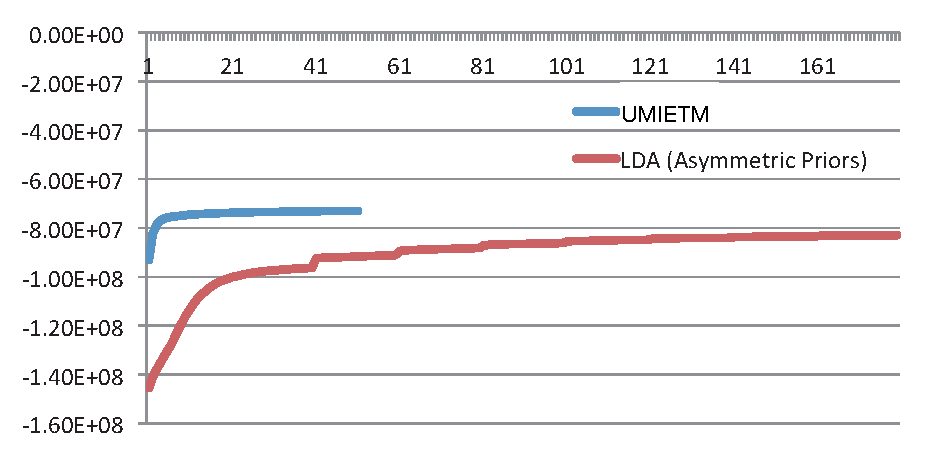
\includegraphics[width=1.0\textwidth]{img/UMIETM/completeLoglikelihood.pdf}
\end{figure}

\end{frame}


%------------------------------
\begin{frame}
\frametitle{实验结果:UMIETM事件检测效率}
\begin{figure}
	\caption{UMIETM在线学习方法用于事件检测的运行效率}
    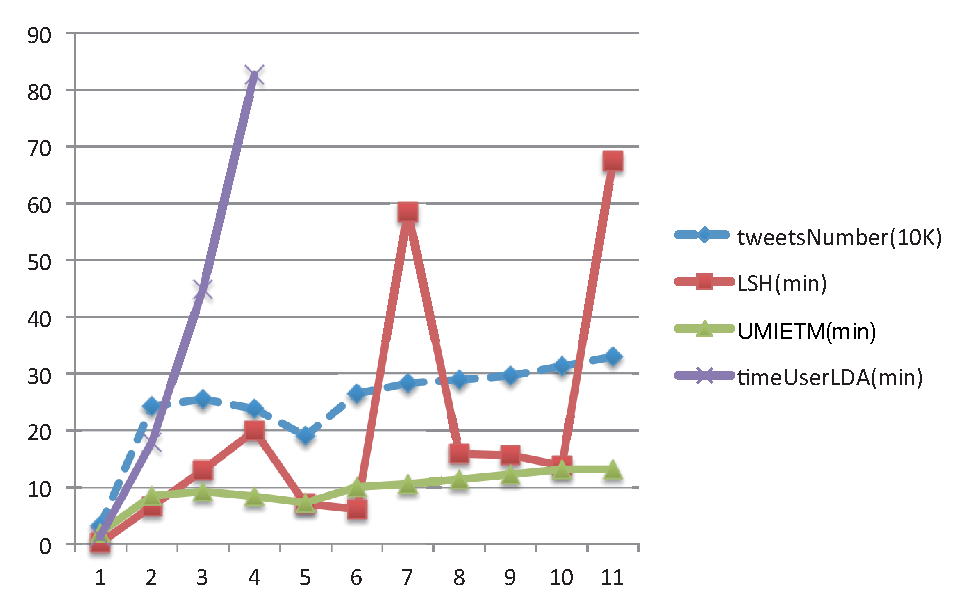
\includegraphics[width=0.8\textwidth]{img/UMIETM/efficiencyCompareWithLSH.pdf}
\end{figure}
\pdfnote{timeUserLDA使用批量学习方法,时间复杂度随着数据集大小线性增长\\ 基于LSH的方法也具备在线学习能力,但时间复杂度不稳定,随着桶内数据大小而变化}
\end{frame}

%------------------------------
\begin{frame}
\frametitle{实验结果:突发事件检测准确率与召回率}

\begin{table}
\centering
\caption{UMIETM与对比方法在新浪微博数据集(2012.1-2012.12)上突发事件检测任务的准确率与召回率比较}
\begin{tabular}{|c|r|r|} \hline
 & precision & recall \\ \hline
UMIETM & 0.894 & 0.913\\ \hline
UMIETM(-) & 0.847 & 0.697 \\ \hline
IETM & 0.824 & 0.536 \\ \hline
LSH & 0.394 & 0.913 \\ \hline
EDCoW & 0.731 & 0.435 \\ \hline
\end{tabular}
\label{tab:metrics}
\end{table}

\end{frame}


%\begin{withoutheadline}
\begin{frame}
\vspace*{-13mm}
\begin{figure}
	\hspace*{-4.2mm}
    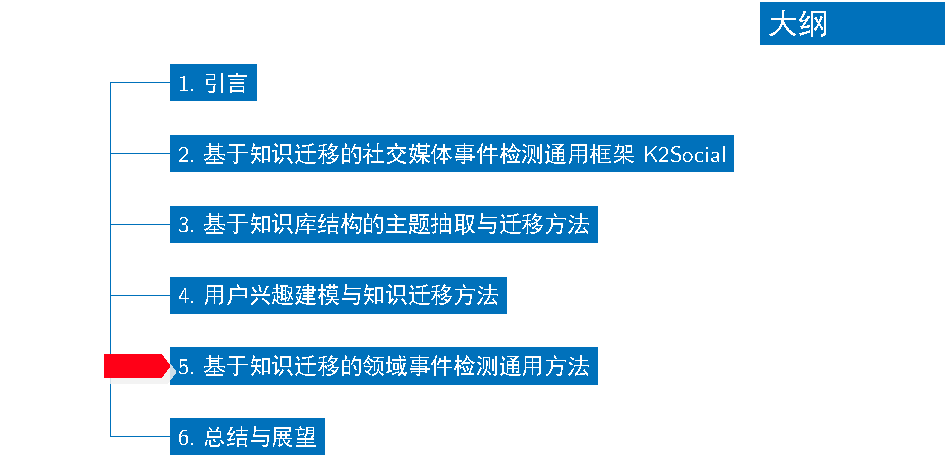
\includegraphics[width=1.0\paperwidth]{img/contents5_output.pdf}
\end{figure}

\end{frame}
\end{withoutheadline}

\section{基于知识迁移的领域事件检测通用方法}
%------------------------------
%\begin{frame}
%\frametitle{Motivation}
%领域事件检测为什么是必须的?
%\pdfnote{有什么合适的例子来说明领域事件检测呢?}
%\end{frame}

%------------------------------
\begin{frame}
\frametitle{领域事件检测与知识抽取的优化}	

\begin{figure}
	\caption{TaxoPhrase用于从维基百科知识库中抽取领域知识的示意图}
    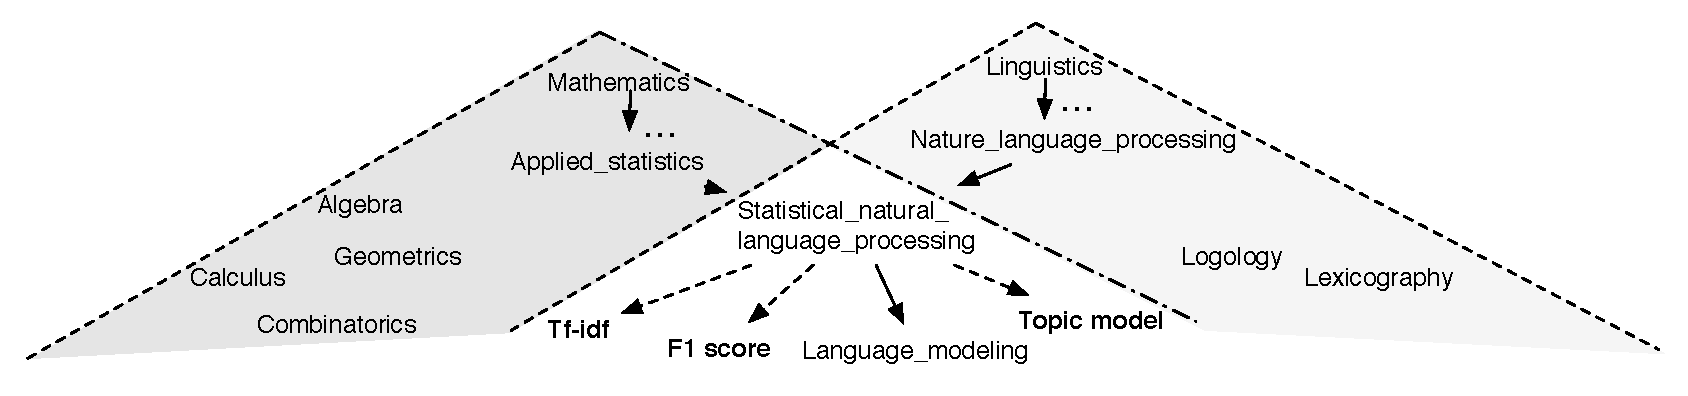
\includegraphics[width=1.0\textwidth]{img/TD+/taxophrase_motivation.pdf}
\end{figure}
\pdfnote{TaxoPhrase用于从知识库中抽取领域知识的示意图。用户1关心\textit{数学}领域中除\textit{统计自然语言处理}(白色区域)之外的知识(深灰色区域),用户2关心\textit{语言学}领域中除\textit{统计自然语言处理}之外的知识(浅灰色区域),在此场景中TaxoPhrase可将上述三部分用主题建模的方法加以探索与抽取。}
\end{frame}

%------------------------------
\begin{frame}
\frametitle{领域事件检测与知识抽取的优化}	
\begin{figure}
	\caption{英文维基百科的分类体系中各类别节点的出度的分布}
    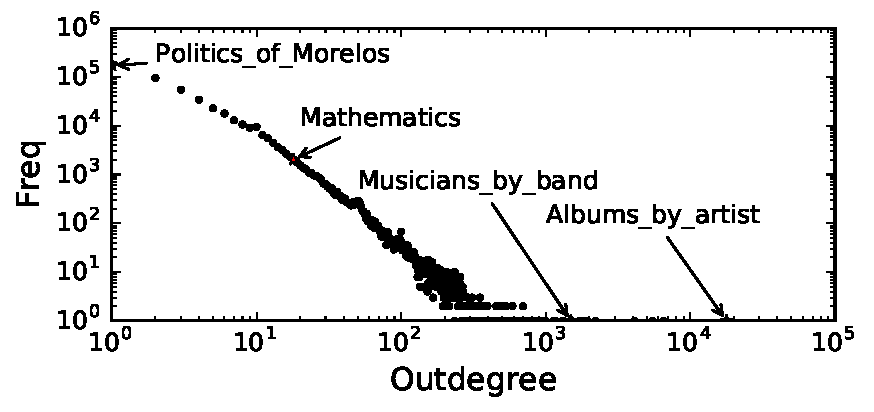
\includegraphics[width=1.0\textwidth]{img/TD+/outdegree_distribution.pdf}
\end{figure}
\end{frame}

%------------------------------
\begin{frame}
\frametitle{领域事件检测与知识抽取的优化}	
\vspace{-5mm}
\begin{figure}
	\setlength{\abovecaptionskip}{0.cm}
	\setlength{\belowcaptionskip}{0.cm}
	\caption{知识库中有互补关系的三部分的示例}
    \includegraphics[width=0.75\textwidth]{img/TD+/example.pdf}
\end{figure}
\pdfnote{可以考虑给图的左侧加上分类类别、实体、短语的标注}
\end{frame}

%------------------------------
\begin{frame}
\frametitle{TaxoPhrase模型}
\begin{figure}
	\centering
	\caption{用于探索知识库中领域知识的概率模型TaxoPhrase的示意图}
    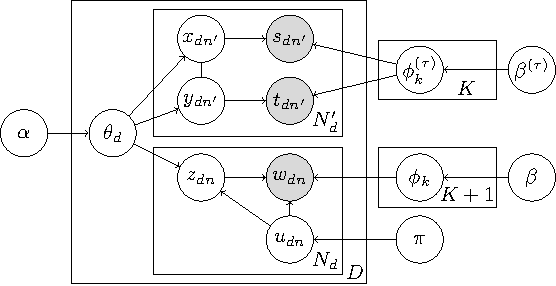
\includegraphics[width=0.8\columnwidth]{img/TD+/TaxoPhrase_inpaper.pdf}
	\label{fig:IllustrationTaxoPhrase}
\end{figure}
\end{frame}


%------------------------------
\begin{frame}
\frametitle{实验结果:TaxoPhrase的建模质量}	
%\begin{table}
%\centering
%\caption{TaxoPhrase方法在Mathematics@Wiki上学得的主题(取规模较大的5个进行展示,\(K\)=100)。\textit{斜体部分}表示分类类别,\texttt{黑体部分}表示实体,普通字体表示短语。五个主题分别对应了数学家与数学奖项,几何学,拓扑学,密码学,代数学。}
%\label{my-label}
%\begin{tabular}{|>{\columncolor[gray]{0.8}}c|c|}
%\hline
%Topic 1 &  \\
%\multicolumn{2}{|p{15.2cm}|}{(Categories) \textit{Mathematics\_awards}, \textit{Mathematicians\_by\_award}, \textit{Mathematicians\_by\_nationality}, \textit{Mathematicians\_by\_field}}\\
%%\hdashline
%\multicolumn{2}{|p{15.2cm}|}{(Entities) \texttt{John Cedric Griffiths Teaching Award}, \texttt{Santosh Vempala}, \texttt{Aisenstadt Prize}, \texttt{Subhash Suri}, \texttt{David P. Dobkin}}\\
%%\hdashline
%\multicolumn{2}{|p{15.2cm}|}{(Phrases) university of california, american mathematical society, professor of mathematics, princeton university, computer science, harvard university, american mathematician, stanford university, massachusetts institute of technology, columbia university}\\
%\hline
%\hline
%Topic 2 &  \\
%\multicolumn{2}{|p{15.2cm}|}{(Categories) \textit{Geometry\_stubs}, \textit{Differential\_geometry\_stubs}, \textit{Elementary\_geometry\_stubs}, \textit{Polyhedron\_stubs}}\\
%%%\hdashline
%\multicolumn{2}{|p{15.2cm}|}{(Entities) \texttt{Enneadecahedron}, \texttt{Icosahedral pyramid}, \texttt{Expanded icosidodecahedron}, \texttt{Pentadecahedron}, \texttt{Cubic cupola}}\\
%%\hdashline
%\multicolumn{2}{|p{15.2cm}|}{(Phrases) three dimensional, platonic solids, johnson solids, uniform polyhedron compound, symmetry group, regular dodecahedron, triangular faces, vertex figure, nonconvex uniform polyhedron, four dimensional}\\
%\hline
%\hline
%Topic 3 &  \\
%\multicolumn{2}{|p{15.2cm}|}{(Categories) \textit{Topology\_stubs}, \textit{Knot\_theory\_stubs}, \textit{Theorems\_in\_topology}, \textit{Theorems\_in\_algebraic\_topology}}\\
%%\hdashline
%\multicolumn{2}{|p{15.2cm}|}{(Entities) \texttt{Knot operation}, \texttt{Chromatic homotopy theory}, \texttt{Infinite loop space machine}, \texttt{Simple space}, \texttt{Base change map}}\\
%%\hdashline
%\multicolumn{2}{|p{15.2cm}|}{(Phrases) topological space, algebraic topology, category theory, topological spaces, fundamental group, simply connected, homotopy theory, 3 manifold, 3 manifolds, knot theory}\\
%\hline
%\hline
%Topic 4 &  \\
%\multicolumn{2}{|p{15.2cm}|}{(Categories) \textit{Cryptography\_stubs}, \textit{Cryptography}, \textit{Combinatorics\_stubs}, \textit{Number\_stubs}}\\
%%\hdashline
%\multicolumn{2}{|p{15.2cm}|}{(Entities) \texttt{PC1 cipher}, \texttt{PKCS 8}, \texttt{KR advantage}, \texttt{Ccrypt}, \texttt{BEAR and LION ciphers}}\\
%%\hdashline
%\multicolumn{2}{|p{15.2cm}|}{(Phrases) dual ec drbg, block cipher, sha 1, public key, hash function, stream cipher, escape wheel, balance wheel, secret key, private key}\\
%\hline
%\hline
%Topic 5 & \\
%\multicolumn{2}{|p{15.2cm}|}{(Categories) \textit{Algebra\_stubs}, \textit{Abstract\_algebra\_stubs}, \textit{Linear\_algebra\_stubs}, \textit{Theorems\_in\_algebra}} \\
%\multicolumn{2}{|p{15.2cm}|}{(Entities) \texttt{C-closed subgroup}, \texttt{Torsion abelian group}, \texttt{Fixed-point subgroup}, \texttt{Change of rings}, \texttt{Acceptable ring}}\\
%\multicolumn{2}{|p{15.2cm}|}{(Phrases) algebraic geometry, group theory, abstract algebra, finite group, finitely generated, abelian group, finite groups, galois group, commutative ring, normal subgroup}\\
%\hline
%\end{tabular}
%\label{tbl:taxophrase_topics}
%\end{table}

\vspace{-7mm}
\begin{figure}
	\centering
	\caption{TaxoPhrase方法在Mathematics@Wiki上学得的主题}
    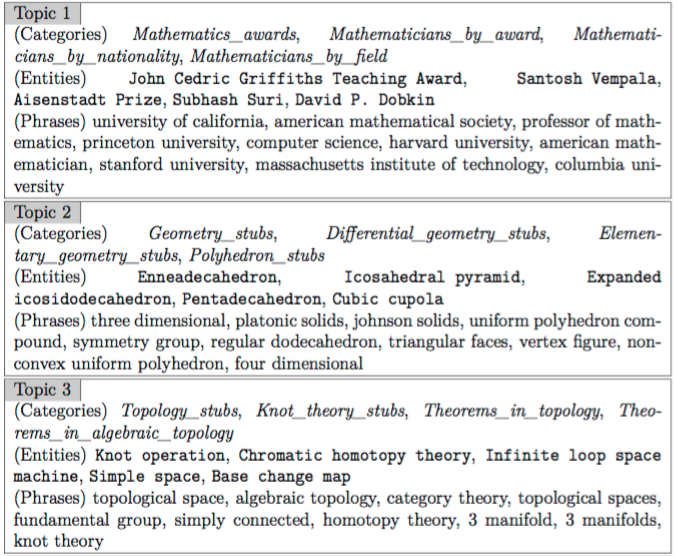
\includegraphics[width=0.8\columnwidth]{img/TD+/topics1.png}
\end{figure}

\pdfnote{加TaxoPhrase在Maths上的建模结果}
\end{frame}


%------------------------------
\begin{frame}
\frametitle{实验结果:TaxoPhrase的建模质量}	

\begin{table}[]
\centering
\caption{各数据集统计信息,以及各方法获得的短语和分类类别两种主题的质量对比(以PMI为评测指标)}
\label{my-label}
\scalebox{0.8}{
\begin{tabular}{p{2.5cm}|l|r|r|r}
\hline
\multicolumn{2}{c|}{}           & Maths & Chemistry & Argentina \\
\hline
\multicolumn{2}{c|}{\#Entities} & 27,947 &  60,375 & 8,617 \\
%\hline
\multicolumn{2}{c|}{\#Category Types}  &     1,391        &3,038&	1,479\\
%\hline
\multicolumn{2}{c|}{\#Phrase Types}     &     116,013        &248,769&     21,183      \\
\hline
\hline
\multirow{2}{*}{on phrases} & LDA  &4.55 & 4.30 & 3.52 \\
&    TaxoPhrase &4.67& 4.55 & 3.81\\
\hline
\multirow{2}{*}{on categories} & SSN-LDA & 4.01 &3.97 &3.06\\
& TaxoPhrase & 4.51 &4.48& 3.73\\
\hline          
\end{tabular}
}
\label{tbl:taxophrase_dataset}
\end{table}
\end{frame}


%------------------------------
\begin{frame}
\frametitle{实验结果:TaxoPhrase抽取领域知识的实例}
\vspace{-7mm}
\begin{figure}
	\centering
	\caption{TaxoPhrase方法在Feminism@Wiki上学得的主题}
    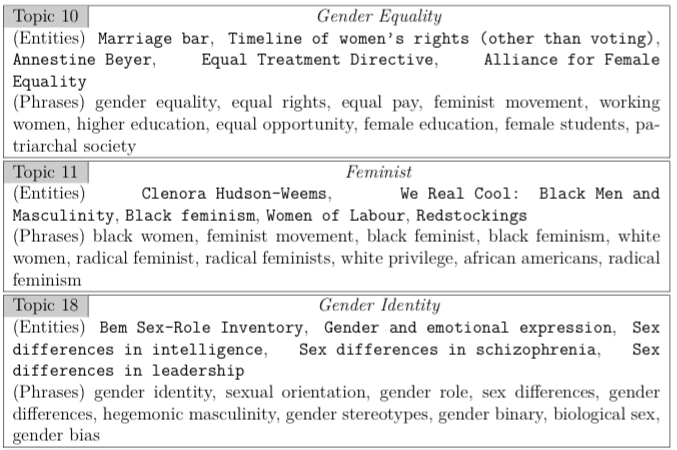
\includegraphics[width=0.8\columnwidth]{img/TD+/topics2.png}
\end{figure}
\pdfnote{加TaxoPhrase在Feminism上的建模结果}
\end{frame}


%------------------------------
\begin{frame}
\frametitle{实验结果:TransDetector$^+$领域事件检测}
\begin{table}
\centering
\setlength{\abovecaptionskip}{0.cm}
\setlength{\belowcaptionskip}{0.cm}
\caption{2011年6月30日至2011年9月15日,\textit{Edinburgh twitter corpus}数据集中Feminist(女权主义)相关事件列表及各事件检测方法在各事件上的具体表现}
\label{my-label}
\scalebox{0.65}{
\begin{threeparttable}  
\begin{tabular}{|c|l|c|c|c|c|c|c|c|}
\hline
\multirow{2}{*}{Date}  & \multirow{2}{*}{Representative event tweet} & \multirow{2}{*}{\begin{tabular}[c]{@{}l@{}}Number of \\ event tweet\end{tabular}} & \multicolumn{6}{c|}{Methods\tnote{a}} \\ \cline{4-9} 
 &  &  & L & TU & TW & E & B & TD+ \\ \hline
7/1/11  & \begin{tabular}[c]{@{}l@{}l@{}}DSK Has Bail Lifted Over \textbf{Sex Assault Case}:\\ Dominique Strauss-Kahn has had his bail\\ lifted after prosecutors said... http://bit.ly/llcWhN \end{tabular} & 46 & - & - & - & - & - & \checkmark \\ \hline
7/26/11 & \begin{tabular}[c]{@{}l@{}}bad! David Wu resigns because of an \textbf{unwanted}\\ \textbf{sexual encounter} with an 18-year-old \end{tabular} & 23 & - & - & - &  - & - & \checkmark  \\ \hline
8/17/11  & \begin{tabular}[c]{@{}l@{}l@{}} Nevin Shapiro said he provided players with \\ \textbf{sexual bribery} and cars over years, and\\ NCAA is investigating http://dlvr.it/cAaMF \end{tabular} & 52 & \checkmark & - & \checkmark & \checkmark & -  & \checkmark \\ \hline
8/19/11 & \begin{tabular}[c]{@{}l@{}l@{}l@{}l@{}} Obama relieves illegal immigrants who are\\ students, veterans, the elderly, crime victims\\ and those with family, including \textbf{same-sex partners} \end{tabular} & 21 & - & -  & \checkmark & - & -  & \checkmark \\ \hline
\end{tabular}

\begin{tablenotes}  
\item[a] L=LSH, TU=TimeUserLDA, TW, E=EDCoW, B=BurstyBTM, TD+=TaxoPhrase+\textsc{TransDetector}
\end{tablenotes}  
\end{threeparttable}  
}
\label{tbl:feminist_event_list}
\end{table}
\end{frame}

%------------------------------
\begin{frame}
\frametitle{实验结果:TransDetector$^+$领域事件检测}
\vspace{-7mm}
\begin{table}[!htbp]
\centering
\setlength{\abovecaptionskip}{2.mm}
\setlength{\belowcaptionskip}{1.mm}
\caption{\textit{Edinburgh twitter corpus}数据集中Natural Hazards(自然灾害)相关事件}
\label{my-label}
\scalebox{0.53}{
\begin{threeparttable}  
\begin{tabular}{|c|l|c|c|c|c|c|c|c|}
\hline
\multirow{2}{*}{Date}  & \multirow{2}{*}{Representative event tweet} & \multirow{2}{*}{\begin{tabular}[c]{@{}l@{}}Number of \\ event tweet\end{tabular}} & \multicolumn{6}{c|}{Methods\tnote{a}} \\ \cline{4-9} 
 &  &  & L & TU & TW & E & B & TD+ \\ \hline
7/2/11  & \begin{tabular}[c]{@{}l@{}l@{}}Exxon \textbf{oil spill} in Mont. river prompts\\ evacuations [AP] - An ExxonMobil pipeline that runs\\ under the Yellowstone River http://tiny.ly/IGuN \end{tabular} & 22 & - & - & - & - & - & \checkmark  \\ \hline
7/5/11 & \begin{tabular}[c]{@{}l@{}l@{}} @438PM Watching \textbf{storms} form around \#Phoenix,\\ potential for a \textbf{dust storm} 6-9PM. \#Tucson about\\ to get hit. \#azwx http://www.weather.gov/phoenix \end{tabular} & 40 & - & - & \checkmark &  - & - & \checkmark \\ \hline
7/11/11  & \begin{tabular}[c]{@{}l@{}l@{}} Possible \textbf{earthquake} east coast of\\ Honshu, JAPON ! 48hrs. close attention. \end{tabular} & 14 & - & - & - & - & - & \checkmark  \\ \hline
7/21/11  & \begin{tabular}[c]{@{}l@{}l@{}} DTN France: Deadly \textbf{heat-wave} spreads in US: A \\punishing \textbf{heat-wave} settles over the central and\\ eastern US, with ... http://bit.ly/q5mRkI. \end{tabular} & 249 & \checkmark & - & \checkmark & \checkmark & - & \checkmark  \\ \hline
8/23/11 & \begin{tabular}[c]{@{}l@{}l@{}l@{}l@{}} More
Virginia \textbf{Earthquake} 2011: Philadelphia\\ Eagles Feel Quake In Locker Room (VIDEO)\\ http://post.ly/2yOQ8 \end{tabular} & 310 & \checkmark & \checkmark  & \checkmark & \checkmark & \checkmark & \checkmark  \\ \hline
8/28/11 & \begin{tabular}[c]{@{}l@{}l@{}l@{}l@{}} @CBSBigBrother Anything but \textbf{Hurricane} \textbf{Irene} \end{tabular} & 1458 & \checkmark & \checkmark  & \checkmark & \checkmark & \checkmark & \checkmark  \\ \hline
9/1/11 & \begin{tabular}[c]{@{}l@{}l@{}l@{}l@{}} \textbf{Tropical storm} Lee in the Gulf of Mexico showed\\ up randomly like at mama's house looking to borrow \\a few dollars. \end{tabular} & 159 & \checkmark & -  & \checkmark & - & - & \checkmark  \\ \hline
9/5/11 & \begin{tabular}[c]{@{}l@{}l@{}l@{}l@{}} Satellite loop of the \textbf{wildfires} in Texas \\ http://fb.me/Zbve5o4E \end{tabular} & 21 & - & -  & - & \checkmark & - & \checkmark  \\ \hline
\end{tabular}

\begin{tablenotes}  
\item[a] L=LSH, TU=TimeUserLDA, TW, E=EDCoW, B=BurstyBTM, TD+=TaxoPhrase+\textsc{TransDetector}
\end{tablenotes}  
\end{threeparttable}  
}
\label{tbl:natural_hazards_event_list}
\end{table}
\end{frame}

%------------------------------
\begin{frame}
\frametitle{TransDetector$^+$方法小结}

\begin{columns}
\column{0.75\textwidth}

\begin{enumerate}
	\item 提出了一种适用于各领域的领域事件检测通用方法TransDetector$^+$;
	\item 提出概率模型TaxoPhrase优化从知识库中抽取领域知识的过程;
	\item TransDetector$^+$将抽取出的领域知识迁移至社交媒体数据流中,检测领域事件;
	\item 在4个示例领域中进行实验,相较于已有方法,平均将F值提升了21\%
\end{enumerate}

\column{0.25\textwidth}

\end{columns}

\pdfnote{本文提出了一种适用于各领域的领域事件检测通用方法TransDetector+。TransDetector+方法利用本文提出的概率模型TaxoPhrase优化从知识库中抽取领域知识的过程,并将抽取出的领域知识迁移至社交媒体数据流中,提取和领域相关的词和短语的时间序列,进而检测领域事件。TransDetector+在4个示例领域中进行了实验,相较于已有方法,平均将F值提升了21\%}

\end{frame}

%\begin{withoutheadline}
\begin{frame}
\vspace*{-13mm}
\begin{figure}
	\hspace*{-4.2mm}
    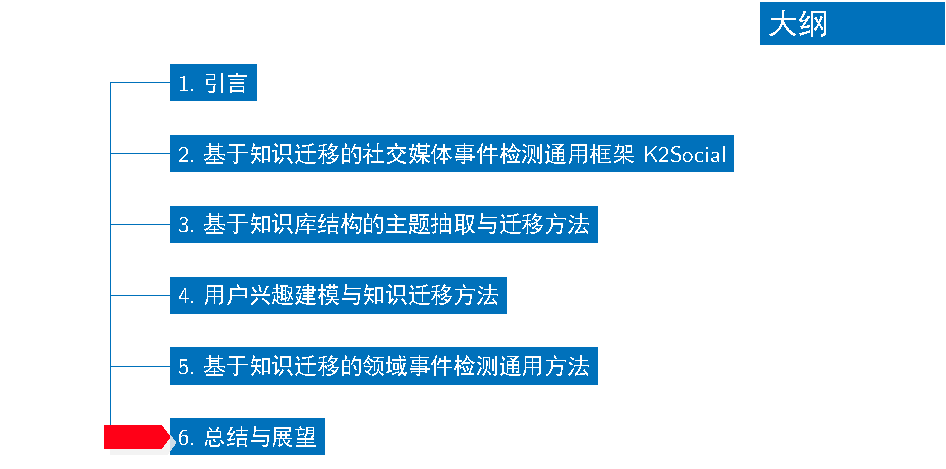
\includegraphics[width=1.0\paperwidth]{img/contents6_output.pdf}
\end{figure}

\end{frame}
\end{withoutheadline}

\section{总结与展望}
%------------------------------
\begin{frame}
\frametitle{总结}
\begin{tikzpicture}[node distance=5mm]
\tikzset{
    every node/.style={draw, rectangle, align=center, text width=3cm, inner sep=0, thick, outer sep=0}
}
\footnotesize
\node[fill=golden, minimum height=4cm, minimum width=3cm, text width=2cm] (one) {基于知识库结构的主题抽取与迁移方法TransDetector};

\node[fill=golden, minimum height=4cm, minimum width=3cm, text width=2cm, right =of one.south east, anchor=south west] (two) {用户兴趣建模与知识迁移方法UMIETM};

\node[fill=golden, minimum height=4cm, minimum width=3cm, text width=2cm, right =of two.south east, anchor=south west] (three) {基于知识迁移的领域事件检测通用方法TransDetector$^+$};

\node[fill=red!40, fit={(one.west) (three.east)}, minimum height=1cm, below =of two] (four) {基于知识迁移的社交媒体事件检测通用框架K2Social};

\node[fill=grassgreen, text=white, fit={(one.west) (one.east)}, minimum height=1.6cm,  above= of one] (a) {提升事件检测准确性,实验中提升9\%};

\node[fill=grassgreen, text=white, fit={(one.west) (one.east)}, minimum height=1.6cm,  above= of two] (b) {提升突发事件检测时效性,实验中提前1.4小时};

\node[fill=grassgreen, text=white, fit={(one.west) (one.east)}, minimum height=1.6cm,  above= of three] (b) {提升领域事件检测准确性,实验中F值提升21\%};

\end{tikzpicture}
	
\end{frame}


%-----------------------------
\begin{frame}
\frametitle{未来工作展望}
\begin{tikzpicture}[node distance=5mm]
\tikzset{
    every node/.style={draw, rectangle, align=center, text width=3cm, inner sep=0, thick, outer sep=0}
}
\footnotesize
\node[fill=grassgreen, text=white, minimum width=10cm, minimum height=1.6cm, text width=10cm] (a) {更多与领域相关的社会计算任务:如心理危机干预,网络亚文化社区检测等};

\node[fill=golden, minimum width=10cm, minimum height=1cm, text width=10cm, below =of a] (one) {扩展面向领域的知识迁移方法};

\node[fill=red!40, minimum width=10cm, minimum height=1cm, text width=10cm, below =of one] (four) {扩展基于知识迁移的社交媒体事件检测通用框架K2Social};

\end{tikzpicture}
	
\end{frame}
%%------------------------------
%page 1
\begin{transparentFootline}
\begin{frame}
\frametitle{\noindent 论文发表情况(1/3)}

\footnotesize
\begin{enumerate}
\item \textbf{Weijing Huang}, Tengjiao Wang, Wei Chen, Siyuan Jiang, Kam-Fai Wong, PhraseCTM: Correlated Topic Modeling on Phrases within Markov Random Fields, ACL 2018, accepted. 
\item \textbf{Weijing Huang}, Tengjiao Wang, Wei Chen, Yazhou Wang, Category-Level Transfer Learning from Knowledge Base to Microblog Stream for Accurate Event Detection, DASFAA 2017. (EI index number: 20174404323179)
\item \textbf{Weijing Huang}, Wei Chen, Tengjiao Wang, Shibo Tao. TaxoPhrase: Exploring Knowledge Base via Joint Learning of Taxonomy and Topical Phrases, the 2nd Open Knowledge Base and Question Answering Workshop at SIGIR 2017.
\item \textbf{Weijing Huang}, Wei Chen, Tengjiao Wang, Shibo Tao. Efficient Topic Modeling on Phrases via Sparsity, the 29th IEEE International Conference on Tools with Artificial Intelligence (ICTAI) 2017. 
\item \textbf{Weijing Huang}, Wei Chen, Lamei Zhang, Tengjiao Wang, An Efficient Online Event Detection Method for Microblogs via User Modeling, the 18th Asia Pacific Web Conference (APWeb) 2016. (EI index number: 20164102880250)
\end{enumerate}
\end{frame}
\end{transparentFootline}

%------------------------------
%page 2
\begin{transparentFootline}
\begin{frame}
\frametitle{\noindent 论文发表情况(2/3)}

\footnotesize
\begin{enumerate}\addtocounter{enumi}{5}
\item Ruhui Wang, \textbf{Weijing Huang}, Wei Chen, Tengjiao Wang, Kai Lei. ASEM: Mining Aspects and Sentiment of Events from Microblog, the 24th ACM International Conference on Information and Knowledge Management (CIKM) 2015.
\item Yue Wang, \textbf{Weijing Huang}, Lang Zong, Tengjiao Wang, Dongqing Yang: Influence maximization with limit cost in social network. SCIENCE CHINA Information Sciences 56(7): 1-14 (2013) 
\item Yue Wang, \textbf{Weijing Huang}, Wei Chen, Tengjiao Wang,Dongqing Yang. Informed Prediction with Incremental Core-based Friend Cycle Discovering, the 12th International Conference on Web-Age Information Management (WAIM) 2011. 
\item 张腊梅,\textbf{黄威靖},陈薇,王腾蛟,雷凯. EMTM:微博中与主题相关的专家挖掘方法. 计算机研究与发展. 2016年(第53卷)(萨师煊优秀学生论文奖).
\item 吴良, \textbf{黄威靖}, 陈薇, 王腾蛟, 雷凯, 刘月琴. ACT-LDA: 集成话题、社区和影响力分析的概率模型. 计算机科学与探索. 2013年第7卷第8期(718-728). 
\end{enumerate}
\end{frame}
\end{transparentFootline}

%------------------------------
%page 3
\begin{transparentFootline}
\begin{frame}
\frametitle{\noindent 论文发表情况(3/3)}

\footnotesize
\begin{enumerate}\addtocounter{enumi}{10}
\item Shibo Tao, Xiaorong Wang, \textbf{Weijing Huang}, Wei Chen, Tengjiao Wang, Kai Lei, From Citation Network to Study Map: A Novel Model to Reorganize Academic Literatures, Big Scholar workshop at WWW 2017.
\item Wei Chen, Lang Zong, \textbf{Weijing Huang}, Gaoyan Ou, Yue Wang, Dongqing Yang, An Empirical Study of Massively Parallel Bayesian Networks Learning for Sentiment Extraction from Unstructured Text, the 13th Asia-Pacific Web Conference (APWeb) 2011. 
\item Xilian Li, Wei Chen, Tengjiao Wang, \textbf{Weijing Huang}, Target-specific Convolutional Bi-directional LSTM Neural Network for Political Ideology Analysis, the Asia Pacific Web and Web-Age Information Management Joint Conference on Web and Big Data (APWeb-WAIM) 2017.
\item Xiao Zhang, Xiaorong Wang, Wei Chen, Jie Tao, \textbf{Weijing Huang}, Tengjiao Wang, A Taxi Gap Prediction Method via Double Ensemble Gradient Boosting Decision Tree, the 2nd IEEE International Conference on Intelligent Data and Security 2017.
\end{enumerate}
\end{frame}
\end{transparentFootline}

%------------------------------
%page 4
\begin{transparentFootline}
\begin{frame}
\frametitle{\noindent 参与科研项目情况}

硕博连读期间参与的项目:
\footnotesize
\begin{enumerate}
\item 非结构化数据管理系统北大部分——国家“核高基”重大专项(2010ZX01042-002-002-02)
\item 海量Web数据结构化内容提取与集成及大型示范应用——国家863计划课题(2012AA011002)
\item 微博用户社区及主题时序方法研究——中国信息安全测评中心合作项目
\item 大数据驱动的航天航空装备创新研发与应用示范——十三五国家重点研发计划课题
%\item 新一代互联网XX系统——国家科技支撑计划课题
%\item 微博XX系统——国家XX部合作项目
%\item 邮件XX系统——国家XX部合作项目
\end{enumerate}

\vfill

\normalsize
硕博连读期间参与的专利:
\footnotesize
\begin{enumerate}
\item 基于交互式文档聚类的信息检索方法及系统, \textbf{黄威靖},于倩,陈薇,王腾蛟,杨冬青,CN103514183A.
\item Web社会网络核心用户信息交互演化分析方法,王悦,\textbf{黄威靖},陈薇,王腾蛟,杨冬青,CN102637182A.
\end{enumerate}

\end{frame}
\end{transparentFootline}



%%------------------------------
%page 1
\begin{transparentFootline_lastpages}
{\setbeamercolor{background canvas}{bg=frenchblue}

\begin{frame}
\frametitle{}
{\color{white}感谢导师王腾蛟教授对我的悉心指导!}
\vfill
{\color{white}感谢关心、支持我的人们!}
\vfill
%{\color{white}黄威靖\\ 2018-06-05}
\end{frame}
}
\end{transparentFootline_lastpages}


%------------------------------
%page 2
\begin{transparentFootline_lastpages}
{\setbeamercolor{background canvas}{bg=frenchblue}

\begin{frame}
\frametitle{}
{\color{white}谢谢各位老师!}
\vfill
%{\color{white}黄威靖\\ 2018-06-05}
\end{frame}
}
\end{transparentFootline_lastpages}

\end{document}
